\documentclass[showtrims,		% Mostra as marcas de corte em cruz
			   %trimframe,		% Mostra as marcas de corte em linha, para conferência
			   11pt				% 8pt, 9pt, 10pt, 11pt, 12pt, 14pt, 17pt, 20pt 
			   ]{memoir}
\usepackage[brazilian,
			% english,
			% italian,
			% ngerman,
			% french,
			% russian,
			% polutonikogreek
			]{babel}
\usepackage{anyfontsize}			    % para tamanhos de fontes maiores que \Huge 
\usepackage{relsize}					% para aumentar ou diminuir fonte por pontos. Ex. \smaller[1]
\usepackage{fontspec}					% para rodar fontes do sistema
\usepackage[switch]{lineno} 			% para numerar linhas
\usepackage{lipsum}						% para colocar textos lipsum
\usepackage{alltt}						% para colocar espaços duplos. Ex: verso livre
\usepackage{graphicx}					% para colocar imagens
\usepackage{float}						% para flutuar imagens e tabelas 		
\usepackage{lettrine}					% para capsulares
\usepackage{comment}					% para comentar o código em bloco \begin{comment}...
\usepackage{adforn}						% para adornos & glyphs
\usepackage{xcolor}					 	% para texto colorido
\usepackage{array}
\usepackage[babel]{microtype}			% para ajustes finos na mancha
\usepackage{enumerate,enumitem}			% para tipos diferentes de enumeração/formatação ver `edlab-extra.sty`
\usepackage{url}					% para citar sites \url
\usepackage{marginnote}					% para notas laterais
\usepackage{titlesec}					% para produzir os distanciamentos entre pontos no \dotfill
\usepackage{textpos}

%\usepackage{makeidx} 					% para índice remissivo

\usepackage{edlab-penalties}
\usepackage{edlab-git}
\usepackage{edlab-toc}					% define sumário
\usepackage{edlab-extra}				% define epígrafe, quote
\usepackage[largepost]{edlab-margins}
\usepackage[%semcabeco, 				% para remover cabeço, sobe mancha e mantem estilos
			]{edlab-sections}			% define pagestyle (cabeço, rodapé e seções)
\usepackage[%
			% notasemlinha 			
			% notalinhalonga
			chicagofootnotes			% para notas com número e ponto cf. man. de Chicago
			]{edlab-footnotes}


% Medidas (ver: memoir p.11 fig.2.3)
\parindent=3ex			% Tamanho da indentação
\parskip=0pt			% Entre parágrafos
\marginparsep=1em		% Entre mancha e nota lateral 
\marginparwidth=4em		% Tamanho da caixa de texto da nota laterial

% Fontes
\newfontfamily\formular{Formular}
\newfontfamily\formularlight{Formular Light}
\setmainfont[Ligatures=TeX,Numbers=OldStyle]{Minion Pro}


% Estilos
\makeoddhead{baruch}{}{\scshape\MakeLowercase{\scshape\MakeTextLowercase{\leftmark}}}{}
\makeevenhead{baruch}{}{\scshape\MakeLowercase{Cantos dos animais primordiais}}{}
\makeevenfoot{baruch}{}{\footnotesize\thepage}{}
\makeoddfoot{baruch}{}{\footnotesize\thepage}{}
\pagestyle{baruch}		
\headstyles{baruch}

% Testes


\begin{document}


%\input{MUSSUMIPSUM}  		% Teste da classe
% Este documento tem a ver com as partes do LIVRO. 

% Fronte da coleção Mundo Indígena
\thispagestyle{empty}
\begin{textblock*}{2.625in}(0pt,0pt)%
\vspace*{-2.4cm}
\hspace*{-2.65cm}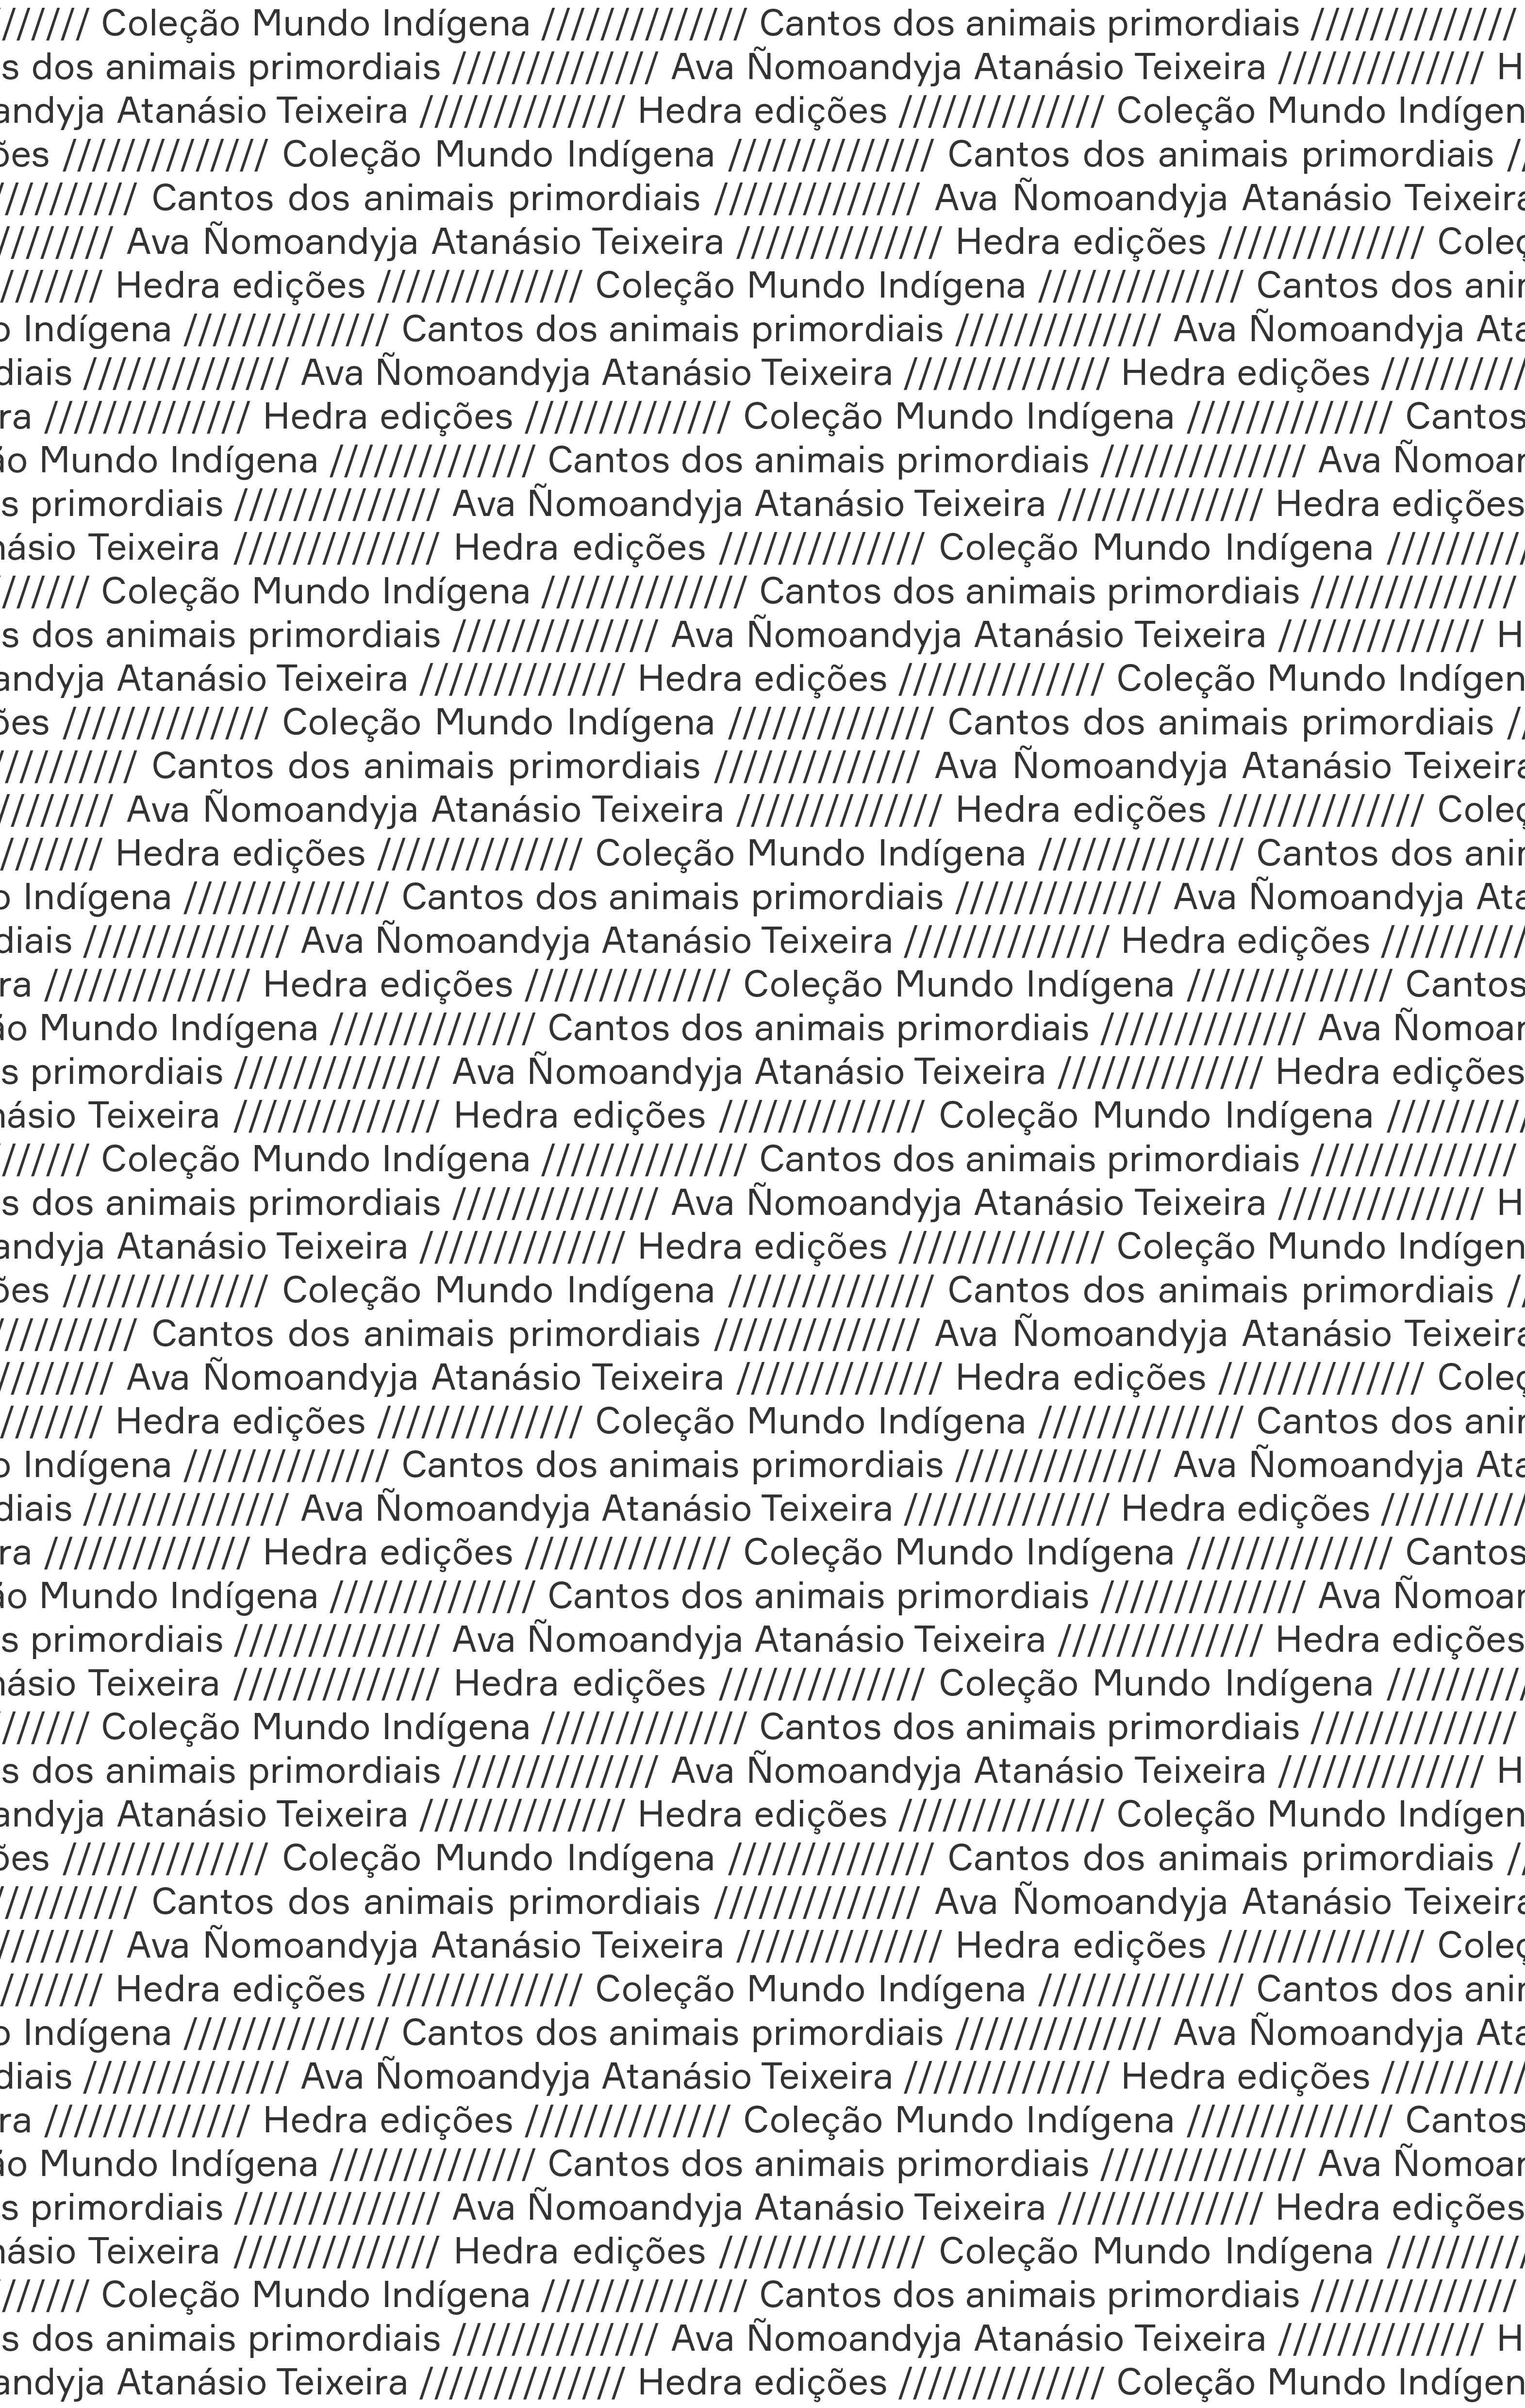
\includegraphics[width=138mm]{./MI_ATANASIO_CANTOS_ABERTURA.png}  
\end{textblock*}
\clearpage
\pagebreak

\thispagestyle{empty}
\begin{textblock*}{2.625in}(0pt,0pt)%
\vspace*{-2.4cm}
\hspace*{-2.3cm}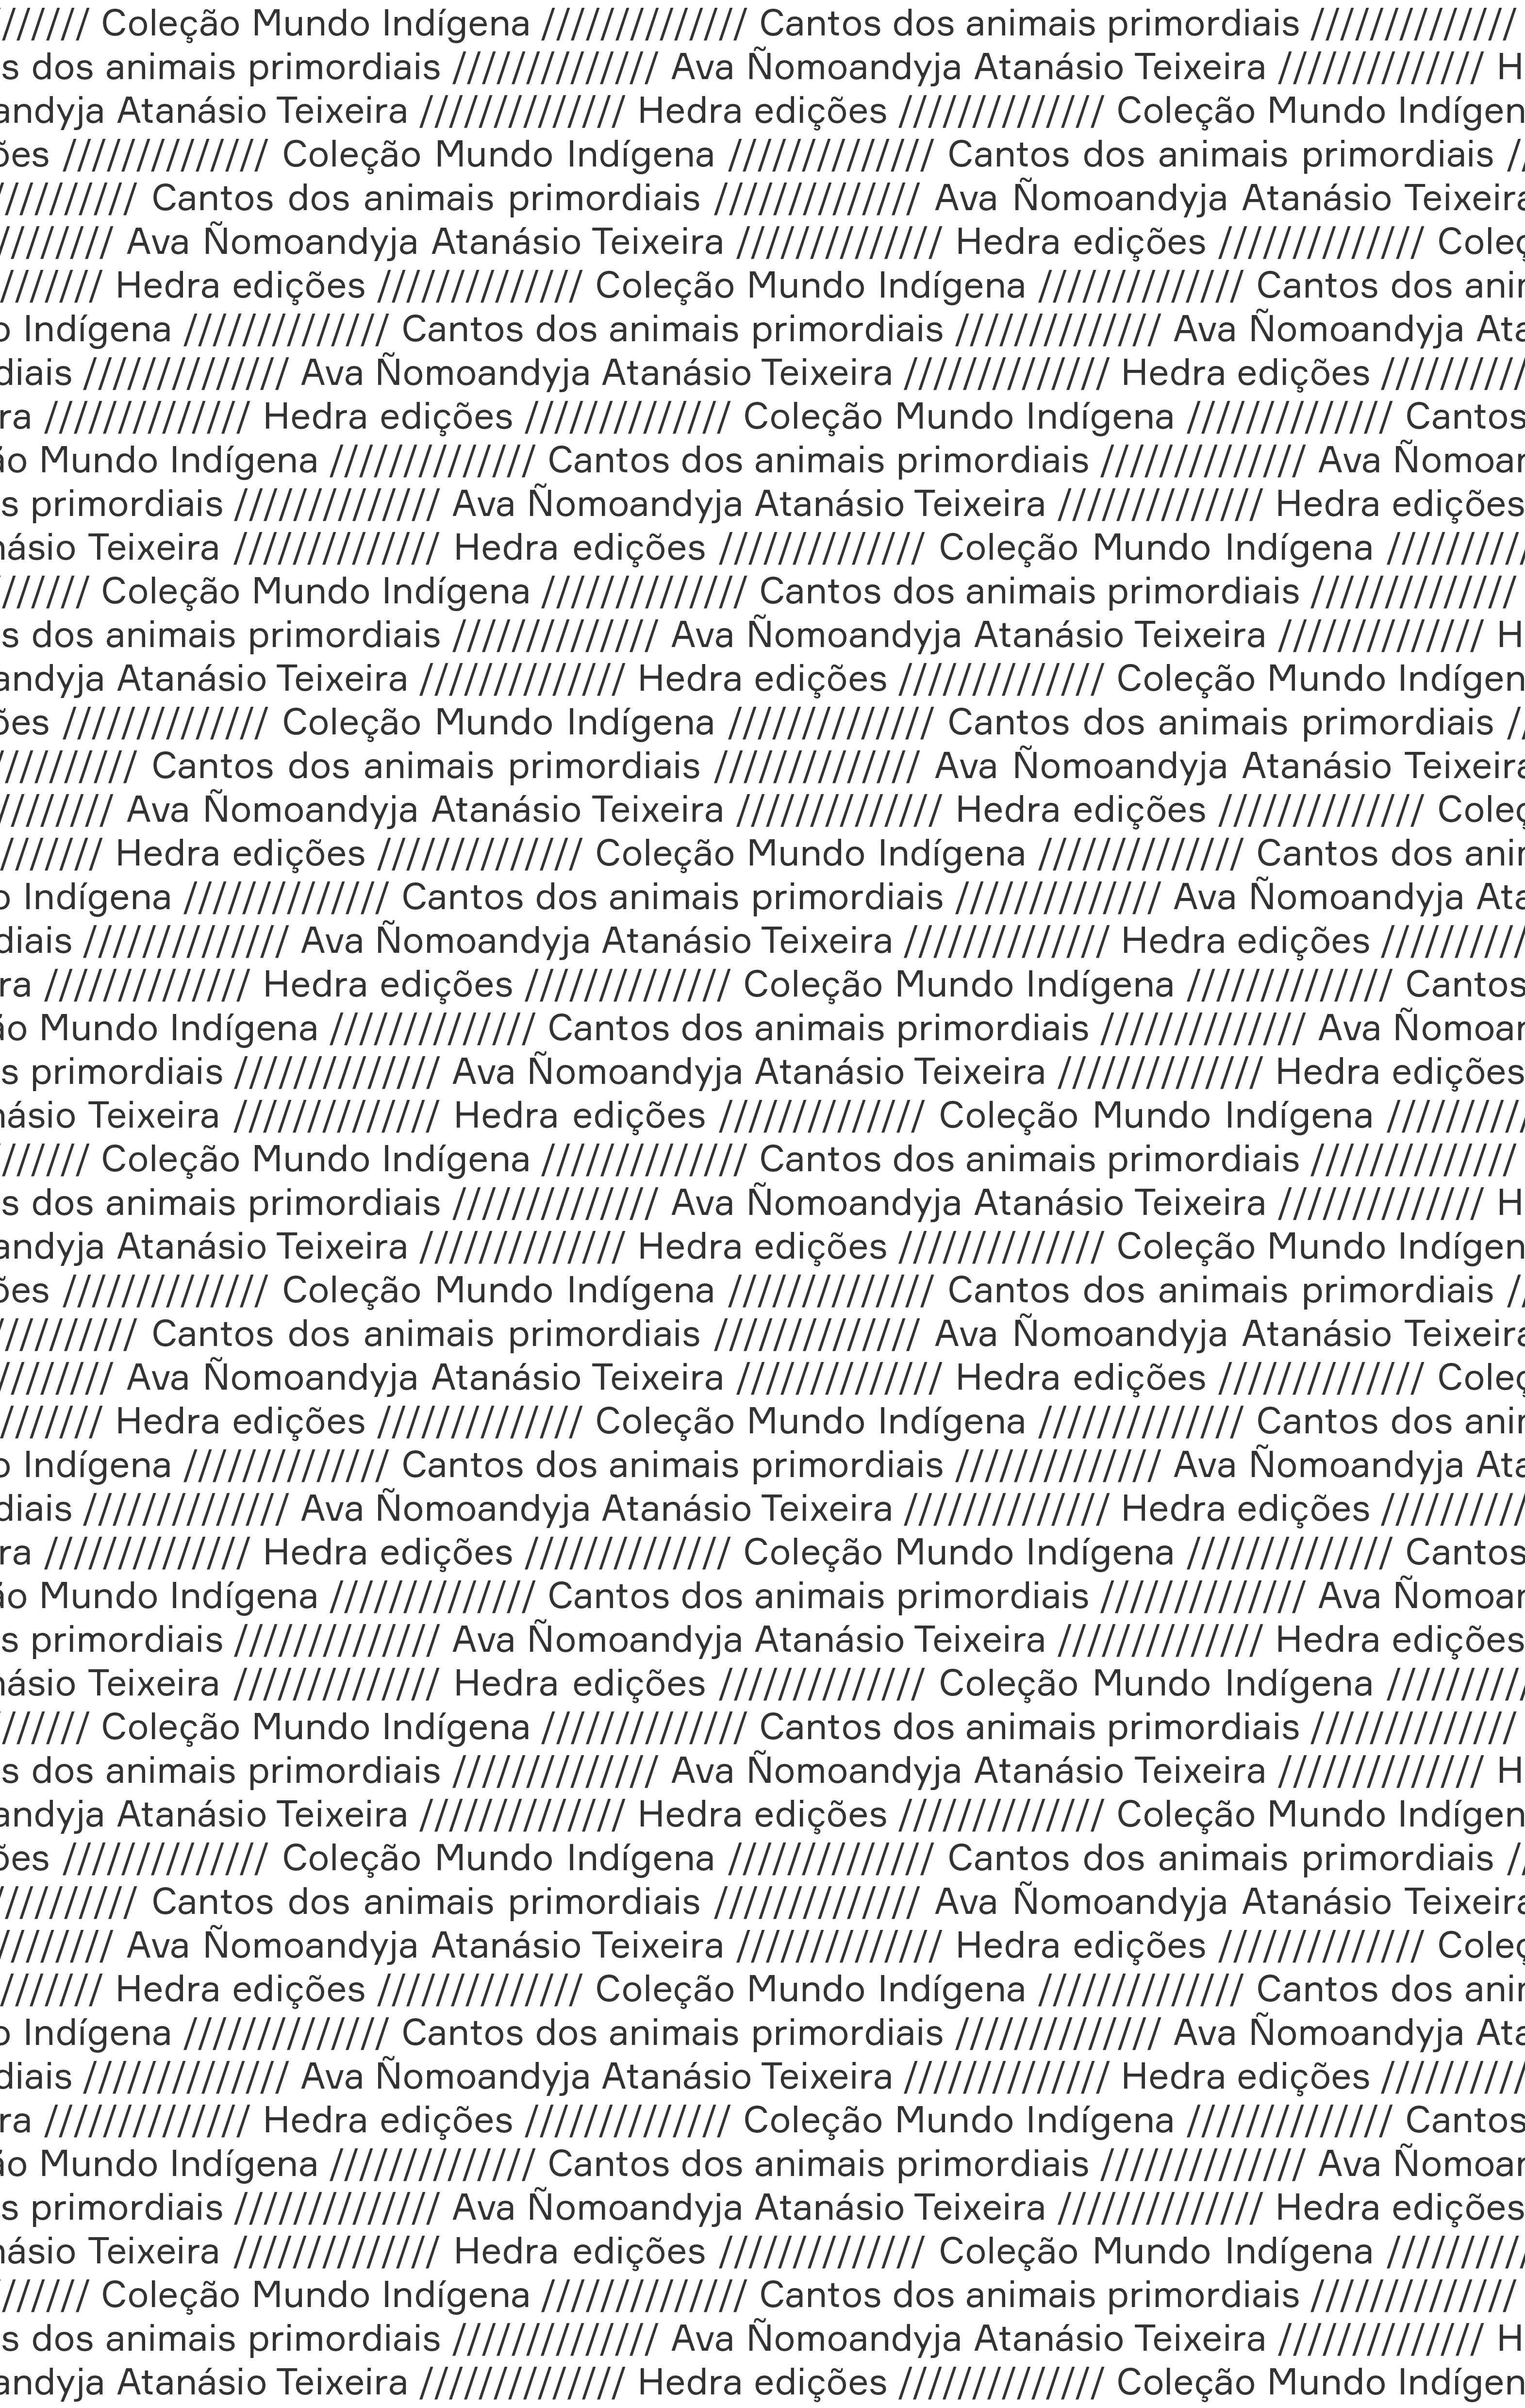
\includegraphics[width=138mm]{./MI_ATANASIO_CANTOS_ABERTURA.png}  
\end{textblock*}
\clearpage

\thispagestyle{empty}

% Tamanhos
% \tiny
% \scriptsize
% \footnotesize
% \small 
% \normalsize
% \large 
% \Large 
% \LARGE 
% \huge
% \Huge

% Posicionamento
% \centering 
% \raggedright
% \raggedleft
% \vfill 
% \hfill 
% \vspace{Xcm}   % Colocar * caso esteja no começo de uma página. Ex: \vspace*{...}
% \hspace{Xcm}

% Estilo de página
% \thispagestyle{<<nosso>>}
% \thispagestyle{empty}
% \thispagestyle{plain}  (só número, sem cabeço)
% https://www.overleaf.com/learn/latex/Headers_and_footers

% Compilador que permite usar fonte de sistema: xelatex, lualatex
% Compilador que não permite usar fonte de sistema: latex, pdflatex

% Definindo fontes
% \setmainfont{Times New Roman}  % Todo o texto
% \newfontfamily\avenir{Avenir}  % Contexto

\begingroup\thispagestyle{empty}\vspace*{.05\textheight} 

              {\formular
              \huge
              \noindent
              \textbf{Cantos dos animais\\primordiais}\\
              
              \vspace{-0.5cm}
              
              \noindent{}{\LARGE Guyra guahu ha mymba\\ ka’aguy ayvu}}
                    
\endgroup
\vfill
\pagebreak       % [Frontistício]
%\newcommand{\linhalayout}[2]{{\tiny\textbf{#1}\quad#2\par}}
\newcommand{\linha}[2]{\ifdef{#2}{\linhalayout{#1}{#2}}{}}

\begingroup\tiny
\parindent=0cm
\thispagestyle{empty}

\textbf{edição brasileira©}\quad			 {Hedra \the\year}\\
\textbf{organização e tradução\,©}\quad	 {Izaque João}\\
\textbf{coorganização\,©}\quad			 	 	 	 {Spensy Pimentel e Tatiane Klein}\\
\textbf{coordenação da coleção}\quad		 {Luísa Valentini}\\

\textbf{edição}\quad			 			 {Suzana Salama}\\
\textbf{assistência editorial}\quad			 {Paulo Henrique Pompermaier}\\
\textbf{revisão do guarani}\quad			 {Arnulfo Morínigo Caballero}\\
\textbf{revisão do português}\quad			 {Spensy Pimentel, Tatiane Klein e Luísa Valentini}\\
\textbf{capa}\quad			 			{Lucas Kröeff}\\

\textbf{ISBN}\quad			 				 {978-65-89705-30-7}\smallskip

\vfill

\begin{minipage}{7cm}
\textbf{Dados Internacionais de Catalogação na Publicação (\textsc{cip})\\
(Câmara Brasileira do Livro, \textsc{sp}, Brasil)}

\textbf{\hrule}\smallskip

Teixeira, Ava Ñomoandyja Atanásio\\

\textit{Cantos dos animais primordiais}. Ava Ñomoandyja Atanásio Teixeira, Izaque João. 1.\,ed. São Paulo, \textsc{sp}: Hedra, 2025.\\


\textsc{isbn} 978-65-89705-30-7\\

1.\,Conto. 2.\,Literatura brasileira. \textsc{i.}\,Teixeira, Ava Ñomoandyja Atanásio. \textsc{ii}.\.Izaque João. \textsc{iii}.\,Título.

\hfill \textsc{cdd}: 869.93

\textbf{\hrule}\smallskip

\textbf{Elaborado por Janaina Ramos (\textsc{crb} 8/\,9166)}\\

\textbf{Índices para catálogo sistemático:}\\
\textsc{i.}\,Conto : Literatura brasileira

\end{minipage}

\vfill

\textit{Grafia atualizada segundo o Acordo Ortográfico da Língua\\
Portuguesa de 1990, em vigor no Brasil desde 2009.}\\

\textit{Direitos reservados em língua\\
portuguesa somente para o Brasil}\\

\textsc{editora hedra ltda.}\\
Av.~São Luís, 187, Piso 3, Loja 8 (Galeria Metrópole)\\
01046--912 São Paulo \textsc{sp} Brasil\\
Telefone/Fax +55 11 3097 8304\\\smallskip
editora@hedra.com.br\\
www.hedra.com.br\\
\bigskip

Foi feito o depósito legal.

\endgroup
\pagebreak     % [Créditos]
% Tamanhos
% \tiny
% \scriptsize
% \footnotesize
% \small 
% \normalsize
% \large 
% \Large 
% \LARGE 
% \huge
% \Huge

% Posicionamento
% \centering 
% \raggedright
% \raggedleft
% \vfill 
% \hfill 
% \vspace{Xcm}   % Colocar * caso esteja no começo de uma página. Ex: \vspace*{...}
% \hspace{Xcm}

% Estilo de página
% \thispagestyle{<<nosso>>}
% \thispagestyle{empty}
% \thispagestyle{plain}  (só número, sem cabeço)
% https://www.overleaf.com/learn/latex/Headers_and_footers

% Compilador que permite usar fonte de sistema: xelatex, lualatex
% Compilador que não permite usar fonte de sistema: latex, pdflatex

% Definindo fontes
% \setmainfont{Times New Roman}  % Todo o texto
% \newfontfamily\avenir{Avenir}  % Contexto

\begingroup\thispagestyle{empty}\vspace*{.05\textheight} 

              \formular
              \Huge
              \noindent
              \textbf{Cantos dos animais primordiais}
              \smallskip
              \noindent\LARGE\textit{Guyra guahu ha mymba ka'aguy ayvu}

              \bigskip  
              
              \LARGE
              \noindent
              Ava Ñomoandyja Atanásio Teixeira
              \vspace{6.8em}
              
              \newfontfamily\minion{Minion Pro}
              {\selectfont\minion\small\noindent Izaque João (\textit{organização e tradução})}


              \bigskip

              \noindent
              {\selectfont\minion\small\noindent 1ª edição}

              \vfill

              \newfontfamily\timesnewroman{Times New Roman}
              {\noindent\fontsize{30}{40}\selectfont \timesnewroman hedra}

              \noindent{\selectfont\minion\small
              \noindent São Paulo \quad\the\year}

\endgroup
\pagebreak
	       % [folha de rosto]
% nothing			is level -3
% \book				is level -2
% \part				is level -1
% \chapter 			is level 0
% \section 			is level 1
% \subsection 		is level 2
% \subsubsection 	is level 3
% \paragraph 		is level 4
% \subparagraph 	is level 5
\setcounter{secnumdepth}{-2}
\setcounter{tocdepth}{0}

% \renewcommand{\contentsname}{Índex} 	% Trocar nome do sumário para 'Índex'
%\ifodd\thepage\relax\else\blankpage\fi 	% Verifica se página é par e coloca página branca
%\tableofcontents*

\pagebreak
\begingroup \footnotesize \parindent0pt \parskip 5pt \thispagestyle{empty} \vspace*{-0.5\textheight}\mbox{} \vfill
\baselineskip=.92\baselineskip
\textbf{Cantos dos animais primordiais} apresenta 26 histórias de aves e outros animais da mata, acompanhados pelos cantos \textit{guahu} que cantam sua história desde o princípio dos tempos. Esses \textit{guahu} fazem parte de um conjunto maior de \textit{cantos-rezas-danças}, conforme denominado pelo xamã e autor, que podemos traduzir como ``cantos míticos''. As narrativas e explicações que acompanham os cantos foram elaboradas por Izaque João, a partir de falas e orientações de Atanásio Teixeira ao longo dos últimos seis anos. Os processos de seleção, transcrição e tradução para esta edição bilíngue também foram feitos em diálogo com o xamã e as versões em português dos textos e cantos \textit{guahu} são um exercício de aproximação a suas belas palavras.

\textbf{Ava Ñomoandyja Atanásio Teixeira} \textls[-10]{(1922--2024) foi um dos mais importantes \textit{ñanderu}, ou ``rezador'', do povo Kaiowá em atividade. Ataná era chamado de \textit{ñamoῖ}, ou ``avô'', por lideranças e rezadores de diferentes comunidades kaiowá, pelos quais ainda é reconhecido como mestre. Foi um dos precursores dos \textit{jeroky guasu}, as ``grandes danças'' dos anos 1980, e do movimento histórico pela recuperação dos territórios kaiowá e guarani em Mato Grosso do Sul, a \textit{Aty Guasu}, ``grande reunião'', além de ser reconhecido como um grande xamã também pelos Guarani. O prestígio de Atanásio está, entre outros motivos, ligado ao fato de dominar as mais variadas técnicas ligadas ao xamanismo kaiowá: os \textit{ñembo'e}, fórmulas verbais de proteção pessoal ou coletiva; os \textit{mborahei} e \textit{guahu}, cantos coletivos ligados aos rituais; os diversos tipos de gestos conhecidos como \textit{jehovasa} --- que podem ser utilizados para influenciar as condições climáticas, desviando tempestades, por exemplo; para curar doenças físicas e espirituais; para garantir a sanidade das lavouras e colheitas etc.}

\textbf{Izaque João}, do povo Kaiowá, é professor e pesquisador dedicado ao estudo dos \textit{cantos-rezas} e conhecimentos tradicionais dos povos Kaiowá e Guarani. Doutorando em
Antropologia na Universidade de São Paulo (\textsc{usp}), é também mestre em História pela
Universidade Federal da Grande Dourados (\textsc{ufgd}). Vive atualmente na Reserva
Indígena de Dourados (\textsc{ms}), onde coordena o Magistério Indígena Ára Verá. Já
coordenou pesquisas para organizações como o Museu do Índio (Funai) e o Fundo
Brasil de Direitos Humanos. É correalizador do documentário \textit{Monocultura da fé} (2018).

\textls[18]{\textbf{Mundo Indígena} reúne materiais produzidos com pensadores de diferentes povos indígenas e pessoas que pesquisam, trabalham ou lutam pela garantia de seus direitos. Os livros foram feitos para serem utilizados pelas comunidades envolvidas na sua produção, e por isso uma parte significativa das obras é bilíngue. Esperamos divulgar a imensa diversidade linguística dos povos indígenas no Brasil, que compreende mais de 150 línguas pertencentes a mais de trinta famílias linguísticas.}




\endgroup

\pagebreak\thispagestyle{empty}\movetooddpage
{\begingroup\mbox{}\pagestyle{empty}
\pagestyle{empty} 
% \renewcommand{\contentsname}{Índex} 	% Trocar nome do sumário para 'Índex'
%\ifodd\thepage\relax\else\blankpage\fi 	% Verifica se página é par e coloca página branca
\addtocontents{toc}{\protect\thispagestyle{empty}}
\tableofcontents*\clearpage\endgroup}

\part{Cantos dos animais primordiais}%\break Guyra guahu ha mymba ka'aguy ayvu}

\chapter*{}
\thispagestyle{empty}
\vspace*{\fill}
\textit{No princípio, chamado pelos Kaiowá e Guarani de \emph{Áraypy}, todas as
aves e animais da mata conversavam uns com os outros, eram considerados
humanos. Um dia, seguindo os irmãos Pa'i Kuara e Jasy, Sol e Lua, na
travessia de um rio, as aves e animais da mata foram derrubados na água
pelo irmão mais novo, Jasy, e foram transformados: nunca mais voltaram a
se entender. Até hoje, cada um deles conta suas origens e seu modo de
ser por meio de um canto \emph{guahu}.}
\vspace*{\fill}

\chapter{O canto da Jararaca}

\letra{A}{} Jararaca é considerada uma criatura monstruosa, por isso essa cobra
possui seu dono. Esse dono da cobra, ao contar sobre o seu jeito de ser,
escondia por completo a sua maldade, falando apenas sobre o ambiente de
sua reprodução e os ovos que estão na extensão de seu corpo.

É verdade que a Jararaca possui vários ovos no seu interior; isso é
contado por meio de seu canto \textit{guahu}. Mbói Jari, no princípio de
sua existência, se esforçou muito para espalhar por toda parte a sua
narrativa de enganosa benevolência, tentando esconder a qualquer custo a
sua maldade. Então ele disse assim: ``Eu também quero deixar para os
seres da Terra o meu canto \textit{guahu}, a ser cantado ao amanhecer.''
Assim disse o dono da cobra, Mbói Jari, e desde então ele deixou o seu
\textit{guahu} aqui na Terra. Por isso o \textit{guahu} da cobra Jararaca só
é cantado no momento do amanhecer; ele fala sobre o ambiente de
reprodução e os ovos que a cobra carrega no seu interior. Essa narrativa
é repassada de geração em geração aos nossos parentes. O \textit{guahu} da
Jararaca é assim:

\begin{verse}
Dono da Jararaca\\
Raiz comprida da árvore,\footnotemark{} lá ela bota seus ovos\\
Dono da Jararaca\\
Raiz comprida da árvore, lá ela bota seus ovos
\end{verse}

Assim é o canto \textit{guahu} da Jararaca.

\footnotetext{``Raiz comprida da árvore'' ou \textit{Yvyra pykue puku} é uma metáfora que a cobra Jararaca utiliza para comparar a extensão do seu corpo com a da raiz das árvores.}

\chapter{Jarara rehegua ñemombe'u}

\letra{M}{bói} mba'e meguã voi, upéagui Jararái jari oipapa jokupe araka'e ogueko
rehegua iguahu yvypórape, ha'e omombe'u oguahu rupi ogupi'a hete
rehegua.


Añetéma, Mbói Jarara oguereko ogupi'a ipuku jave voi oñesyrũ rete rehe;
upéa va'e Jararái omombe'u oguahu rupi. Mbói Jari ypy niko oñeha'ã
mbarete voi araka'e omoherakuã haguã ojehegua iporãeteha, ndaikatúi
mante oipapa ojehegua rekotee rupi, upéagui Mbói Jari omombe'u jokupe ha
upéicha araka'e he'i: ``Che ahejáta ave che guahu yvypórape ko'ẽ ko'ẽ
rupi jeguahu hápy oñeha'ã haguã.'' He'i mbói jary, upéicha oguahu Jarara
ypy omboyvypóry araka'e. Upéagui jeko Jarara guahu oñeha'ã ko'ẽ rupi
mante, oipapa hesegua hupi'a ipuku jave oĩmeha reterehe. Kóa guahu
oipapáva Jarara rehegua iporã jaikuaa ñamombe'u joapýri pýri haguã ñande
kénte kuérype. Jarara guahúko yvy pype he'i:

\begin{verse}
Jarara ri jari\\
Yvyra pykue puku aja katu nde rupi'a\\
Jarara ri jari\\
Yvyra pykue puku aja katu nde rupi'a
\end{verse}


Upéicha Jarara guahu oiko yvypóra ramo.


\chapter{O canto da Perereca}

\letra{P}{erereca}\footnote{Os Kaiowá têm sua própria forma de classificação dos
  anfíbios. \textit{Ju'i gueῖ} é o termo utilizado para se referir às
  pererecas, que podem ser encontradas nas cores verde, amarela e cinza
  nos territórios kaiowá. Já \textit{ju'i mbui}, que é chamada no
  português dos Kaiowá de rã, é maior, é comestível e tem outro tipo de
  canto, assim como seu próprio \textit{guahu}. Existem outras, como por
  exemplo: \textit{ju'i}, uma rã comestível menor que \textit{ju'i mbui},
  comum na região do Ka'aguyrusu; \textit{ytu}, um sapo muito pequeno que
  vive na terra, em locais úmidos, mas frescos, e que pode ser ouvido a
  longas distâncias; \textit{ju'i kara}, uma perereca menor do que
  \textit{ju'ῖ gueῖ} e que se diferencia por meio de seu canto.} de cor
verde, chamada pelos Kaiowá de \textit{ju'i guéĩ}, no princípio da vida,
também fez questão de deixar o seu canto \textit{guahu} para os seres da
Terra, conforme a sua voz e seu jeito de cantar. Perereca, para cantar,
sobe no tronco da árvore e fica bem posicionada. De lá, Perereca canta
sobre seu jeito de ser, assim:

\begin{verse}
\textit{Guéῖ guéῖ}\\
Canta a Perereca\\
\textit{Guéῖ guéĩ}\\
Canta a Perereca\\
No tronco da árvore, canta a Perereca

\textit{Guéῖ guéῖ}\\
Canta a Perereca\\
\textit{Guéῖ guéῖ}\\
Canta a Perereca\\
No tronco da árvore, canta a Perereca
\end{verse}

No momento em que a Perereca canta, onde ela está? Difícil perceber ---
pode estar escondida atrás do tronco da árvore. Perereca canta na
véspera da chuva ou, por meio de seu canto, chama a chuva. Faz todo o
possível de chamar a chuva. Desde então, o \textit{guahu} da Perereca é
cantado em algumas noites, depois de rituais importantes.

\chapter{Ju'i guéῖ guahu}

\letra{J}{u'i} guéῖ ymã ñande ypy reko ñeypyrũ ramo araka'e ko yvy ári, ju'i oheja
oñe'ẽngáry guahu gueko etépygua oñeha'ã haguã yvy pýpe. Ju'i guéῖ niko
he'i oñe'ẽngáry rupi omombe'u yvyraku'a ku'ahápy oiko'akue oguenohẽ
oguahu rupi he'i:


\begin{verse}
\textit{Guéῖ guéῖ}\\
Ere Ju'i\\
\textit{Guéῖ guéĩ}\\
Ere Ju'i\\
Yvyra ku'a peῖ ereñe'ẽko Ju'i
        
\textit{Guéῖ guéῖ}\\ 
Ere Ju'i\\
\textit{Guéῖ guéῖ}\\
Ere Ju'i\\
Yvyra ku'a peῖ ereñe'ẽko Ju'i 
\end{verse}

Upéicha ojehe ju'i he'i. Ju'i niko jasareko ramo hese oñe'ẽ haguã ojupi
voi yvyraku'ápy ha upérupi oñendu uka uka arã oky haguã ikatueteháicha
ohenói amápe. Upéagui pyhare pukukue jeho guahuhápy oñeha'ã mante voi
ju'i guahu oheja iñe'ẽngaryháicha.

\chapter{O canto da Cutia}

\letra{N}{o} início da existência, Cutia recebeu orientações imprescindíveis para
sua vida; depois disso, ela surgiu e se multiplicou aqui na Terra. Cutia
sabe como se desviar da situação perigosa no mato. Cutia possui
inteligência natural e sabe como desarmar armadilha quando é colocada em
seu caminho. Cutia, ao andar na mata, observa atentamente qualquer
madeira pendurada, por isso não é fácil de capturar no mundéu. Esta
história o nosso avô contava bem, sobre o modo de ser da Cutia: antes de
caminhar pela mata, Cutia faz os gestos do \textit{jehovasa},\footnote{\textit{Jehovasa}
  se refere um conjunto de gestos feitos com as mãos, por meio dos quais
  se podem obter diferentes efeitos, como afastar, atrair extirpar,
  proteger, entre outros, a depender do movimento feito pelas mãos.
  Trata-se de uma prática de difusão ampliada, conhecida pela maioria
  das pessoas, mas também empregada de forma especializada pelos
  \textit{ñanderu}, por exemplo nos processos de cura --- quando pode ser
  acompanhado pelo sopro (\textit{peju}). Cutia, da mesma forma, faz
  \textit{jehovasa} não só para escapar do mundéu, mas para afastar todo e
  qualquer mal.} desviando todos os males de seu caminho. Só depois de
fazer \textit{jehovasa}, Cutia sai caminhando no meio da mata, sempre
observando atentamente os arredores. Por esse motivo os Kaiowá, quando
fazem armadilha no trilheiro de Cutia, depois de pronto o mundéu, buscam
o galho com espinhos de uma planta chamada \textit{ñandy ta’y}. Com ele,
golpeiam levemente a armadilha e só depois suspendem a madeira, deixando
ela pronta para capturar a Cutia. Segundo o conhecimento kaiowá, o
mundéu, depois de golpeado com o \textit{ñandy ta’y}, deixa de fazer ruído,
e Cutia não percebe que é armadilha: só assim é que se captura a Cutia. Caso ainda continue a escapar do mundéu, é preciso pegar um punhado da terra por onde Cutia passou e jogá-lo debaixo do mundéu. Só depois de fazer isso é que Cutia entrará na armadilha. Por isso, Cutia, com seu canto \textit{guahu}, fala de sua esperteza,
debochando da aparência do mundéu. Ela canta assim:

\begin{verse}
\textit{Gua ke ke}\\
\textit{Gua ke ke}\\
Escapando do mundéu\\
Escapei do mundéu\\
Escapei do mundéu

\textit{Gua ke ke}\\
\textit{Gua ke ke}\\
Escapando do mundéu\\
Escapei do mundéu\\
Escapei do mundéu  
\end{verse}

Assim o \textit{guahu} da Cutia conta sobre ela.

\chapter{Akutipáy guahu}

\letra{A}{kuti} reko ypy rehegua ñemombe'upy, ha'e niko ohekokuaa araka'e
rembypyrã, ha upérupi ombojehu ha ombojeroreta yvypýpe. Akuti ka'aguy
rupi oiko kuaa voi, ombogua kuaa monde hape rupi ojejapo ramo, hesa katu
yvyra guyrehe, ha upéagui ndoikereíry monde guýpe. Ñande ramõi vete
omombe'u va'ekue rupi ete akuti reko rehegua; ha'e osẽ oguata ha okaru
haguã ka'aguy rupi ojehovasa rañe katuete opa mba'e va'i omboguakatu
raguã oguapegui, ha ojehovasa rire katu oguatáma ka'aguy rupi ha
oñangareko voi opamba'e rehe. Upéagui, monde ojejapo ramo akuti rape
rupi ka'aguy mbyte rupi, monde japoha oinupã nupã rañearã ñandy ta'ypy
ha uperire katu oñakã upi haguã mondépe, upéa rire ndaje monde
ndaijayvúiry akuti oúramo hupi. Ha upéicha háguy ombovy joty ramo monde,
akuti pypore yvy reheve ombohasa arã monde guykoty, upéicha rire mante
ha'e oike monde guýpe. Upéagui akuti oguahu rupi oipapa ñembohory hápy
monde ombogua va'ekue rehegua, ha upéicha he'i:\looseness=-1

\begin{verse}
\textit{Gua ke ke}\\
\textit{Gua ke ke}\\
Monde mogua rire\\
Amoguáko monde ju\\
Amoguáko monde ju
       
\textit{Gua ke ke}\\
\textit{Gua ke ke}\\
Monde mogua rire\\
Amoguáko monde ju\\ \EP[1]
Amoguáko monde ju 
\end{verse}

Upéicha Akuti guahu oipapa ojehegua.

\chapter{O canto da Tartaruga}

\letra{T}{artaruga} e Onça, segundo contam os Kaiowá, se casaram. Depois da
criação do céu e da terra, a Onça fêmea e a Tartaruga macho ficaram
encantados um pelo outro, os dois se apaixonaram perdidamente e se
casaram. Tartaruga anda muito devagar e seu casco é muito duro. Ele não
pode caminhar rápido, a sua pata é arrastada pelo chão, caminha como se
estivesse se arrastando, este é seu jeito de ser, certamente não tem
condições de subir na árvore. A Onça amava o Tartaruga imensamente, não
podia ficar longe dele. Um dia Onça e Tartaruga foram caçar, levando
arco e flecha. Tartaruga, em certo momento, atirou em um pássaro, mas a
sua flecha ficou presa num galho de árvore. Tartaruga tentou subir no
tronco da árvore de cabeça para baixo e não conseguiu. A Onça percebeu
que seu marido Tartaruga não podia subir na árvore, então subiu
rapidamente no tronco da árvore e desprendeu a flecha do galho,
deixando-a cair no chão. Depois desse episódio, Tartaruga ficou muito
envergonhado, olhou seu corpo e percebeu que não podia andar como a sua
esposa. Depois disso, Tartaruga abandonou a sua esposa Onça e foi embora
bem longe. A Onça ficou bastante preocupada e seguiu Tartaruga até o
lugar onde vivia seu amado, gritando e gritando e chamando o nome de
Tartaruga. Em certo momento, Tartaruga ouviu os gritos, e então cantou:

\begin{verse}
Traga-me meu \textit{tembetá}, minha mãe\\
Traga-me meu \textit{tembetá}, minha mãe\\
Traga-me meu \textit{tembetá}, minha mãe\\
Traga-me meu \textit{tembetá}, minha mãe

\pagebreak
Vou lá ver\\
Aquela mulher que eu abandonei\\
Ajoelhada no tronco do Juqueri\footnotemark{}\\
Mulher que não quer entender

Vou lá ver\\
Aquela mulher que eu abandonei\\
Ajoelhada no tronco do Juqueri\\
Mulher que não quer entender
\end{verse}

\footnotetext{Neste verso a Tartaruga fala da Onça, a mulher que insiste
  no homem que a abandonou. O Juqueri é uma árvore de tronco espinhoso,
  então o verso metaforiza os sofrimentos dessa mulher amargurada, que
  não quer se afastar desse homem.}

Onça e Tartaruga se encontraram novamente na beira de um rio. Tartaruga, fugindo de sua mulher, se atirou na água e ficou submerso por alguns minutos. A Onça também se atirou atrás de Tartaruga, mas quase se afogou na água.
Desde então, a Onça fêmea resolveu se separar para sempre de Tartaruga,
pois a Onça não quer morrer só por causa de Tartaruga.

\chapter{Karumbe guahu}

\letra{K}{arumbe} ha jaguarete omenda ramo guare rehegua ñemombe'u. Ary ha yvy
oñepyrũ ha omboypy rire araka'e, jaguarete kuña ha karumbe kuimba'e
oñemboki ete araka'e ojoehe ha omenda, karumbe iguaná eterei ha oguata
mbegue ave, ijape katu ipekue hatã voi. Karumbe ndaikatúi oguata pya'e,
ipy ha ipo yvyrehe opoñy haguánte voi; upéagui ndaikatu mo'ãi voi ojupi
yvyvra rehe, ha jaguarete kuña katu ohayhu eterei ichupe, ndoikoséi
mombyry karumbégui. Peteĩ árype karumbe oho omangeko oguembireko ndive,
oñyvõ ñyvõ guyra yvategua ha iju'y opita ojepoko yvyra rakã rehe,
karumbe ojeupita mo'ã oguevivy iju'y rehe ha ndaikatúi ojeupi, ha
rembireko katu pya'epy ojeupi yvyra rehe omotyvõ oity karumbe hu'y
yvýpy. Upéa rire Karumbe opyta oñemotĩ eterei, ha ojesaity ojehe
ndaikatuiha oiko oguembireko oikoháicha. Upéagui karumbe oheja jaguarete
kuñápe, ha okañỹ mombyry oho guembirekógui. Jaguarete katu ohayhu
etereígui oho hapykuéri oheka karumbépe rekuaty kuaty rupi oñendu'uka
uka karumbépe, upe maramo karumbe oguahu rupi he'i:

\begin{verse}
Eru che rembeta chévy ha'i\\
Eru che rembeta chévy ha'i\\
Eru che rembeta chévy ha'i\\
Eru che rembeta chévy ha'i

\pagebreak       
Taha tahecha\\
Aipo kuña chehegui poindare\\
Guetyma jukeri'y jepe\\
Kuña ndoikuaái
       
Taha tahecha\\
Aipo kuña chehegui poindare\\
Guetyma jukeri'y jepe\\
Kuña ndoikuaái
\end{verse}


Upéicha ha'ekuéry ojotopa jevy y rembe'ýpy, Karumbe katu oguembirekógui 
ojepoi ýpy ha oyguy, ha Jaguarete ojepoi ave hapykuéri ha haimete omano
y guýpy, Jaguarete nomanoséi Karumbe rehehápy opoi ete karumbégui.

\chapter{O canto da Capivara}

\letra{C}{apivara}, conforme a narrativa kaiowá, possui sua história, e ele mesmo
conta sobre o seu ambiente de vida. Capivara narra por meio do canto
\textit{guahu} para as divindades narrativas para repassar de geração a
geração, em cada território. Capivara conta sobre seu ambiente de vida,
algo que é visível nas beiras de rio ou lagos por onde anda. Capivara
gosta de viver na beira da água ou lago, onde é sempre limpo e existe
muita lama, ou poeira, onde Capivara se deita para descansar. Capivara
gosta de comer capim novo e gosta de viver na beira da água ou no brejo,
mas, quando percebe o perigo ou é atacado pelo caçador, corre e cai na
água, ficando por alguns minutos debaixo d'água. Às vezes, sai do outro
lado do córrego e vai embora. No lugar onde vive, a água sempre fica
suja, pois a capivara a todo o momento cai n'água, ou às vezes deixa a
água espumando. Por isso, Capivara, por meio de seu canto \textit{guahu},
narra como é seu ambiente e como brinca com seus companheiros, cantando
assim:

\begin{verse}
No imenso pó da terra eu brinco\\
Espumas d'água eu lanço\\
Espumas d'água eu lanço

No imenso pó da terra eu brinco\\
Espumas d'água eu lanço\\
Espumas d'água eu lanço
\end{verse}

\chapter{Kapiyva guahu}

\letra{K}{apiyva} ypy oipapa ijehegua omombe'u yrykóta rehe guare. Kapiyva oipapa
ogueko rehegua oguahu rupi ñande rembypy kuérype araka'e, ñemombe'u pyrã
voi yvypórape ojeroeta opa tetã guasu hárupi guarã. Kapiyva ogueko
rehegua tesa rupi guarã voi oipapa, mba'éichapa rekuaty ojekuaa va'erã
yrykóta rehe yugua rusu rusu oikoha raty rupi. Kapiyva niko ojehesaity
ha ovy'avéva yugua rusu kóta rehe voi, ha upéagui ha'e oipapa omboyvy
ku'i ku'i oñenoháty oikóvy ramogua. Kapiyva oikoha rupi niko yugua rusu
rembe'y ipotῖ voi, ha'e iñenõha yrykóta ha ikaruháty rupi ndahokýi
ñahãna ra'y, ha'e voi ho'u kapi'i kyre ogueta reheve, upéagui omopotῖ
oguekuaty. Kapiyva oikoeteve yrykóta rehe ha juvy'y rehe, ha ohendu
hapykuéri jeiko ramo, ohepy haguã oguekove ha'e ho'a ave ýpy ha oyta
yguy rupi mombyryhápy osẽ okañy haguã juvy'y rehe. Ha yugua guasu
ojahuháty py katu omohypytĩarã y, ojahu ha ojavyky etereígui ombohyjúi
hyjúi y syry. Upéagui kapiyva oguahu rupi oipapa oguekoha ha oguekuaty
rehegua, ha upéicha he'i:

\begin{verse}
Yvy ku'i guasu rupi che guahapa\\
Yryjúipy ajoapi\\
Yryjúipy ajoapi\\

Yvy ku'i guasu rupi che guahapa\\
Yryjúipy ajoapi\\
Yryjúipy ajoapi
\end{verse}

\chapter{O canto da Lontra}

\letra{P}{or} meio de seu canto \textit{guahu}, Lontra conta seu comportamento e
como vive com outro animal. Como Lontra caça os peixes para comer, pois
gosta de comer peixe de qualidade, seu dente é uma flecha letal para
matar peixe --- as divindades deram uma flecha para seu uso de
sobrevivência. Por esse motivo, por onde Lontra vive e come só os peixes
deixa espalhada a escama de peixe na beira do córrego ou rio só para
demonstrar que come bem e sabe capturar os peixes. {[}Por{]} essas
provocações os outros animais que também comem peixe não gostam de
Lontra. Lontra também gosta de fazer outras provocações: por sua
natureza, Lontra gosta de ter várias fêmeas como suas companheiras,
vivendo em grupo. Cada lontra possui o seu território para viver com
várias lontras fêmeas. O macho caça mais para as fêmeas comerem. Por
isso, Lontra provoca os outros bichos, dizendo que só ele tem várias
esposas e outros não têm. Lontra também às vezes rouba fêmeas de outro
grupo e assim fica feliz vivendo no seu território. A flecha de Lontra é
seu dente, e ele se considera o melhor caçador de peixes de todos os
tempos. Este é o seu jeito, que orgulhosamente narra por meio de seu
canto \textit{guahu}.

\begin{verse}
Eu sou um bom caçador\\
Eu sou um bom caçador

Todos falam de mim\\
\textit{Suas esposas são muitas}\\
Todos falam de mim\\
\textit{Suas esposas são muitas}

\pagebreak
Eu sou um bom caçador\\
Eu sou um bom caçador

Todos falam de mim\\
\textit{Suas esposas são muitas}\\
Todos falam de mim\\
\textit{Suas esposas são muitas}\\
Todos falam de mim\\
\textit{Suas esposas são muitas}

Eu sou um bom caçador\\
Eu sou um bom caçador
\end{verse}

\chapter{Guairaka guahu}

\letra{G}{uairaka} oguahu rupi oipapa ojehegua omoherakuã yvypórape oguekóypy.
Guairaka rembi'u niko pira añónte voi, pira rehe ha'e ojeporeka kuaa y
rupi okaru haguã; upe hekorã hembypy araka'e omboypy ichupe. Upéagui
ikaruhaty hague rupi y rembe rehe hetave hetave pira pekue omosãrambi.
Upéichagui guairaka ojehegua omombe'u ha oñemomba'e guasu voi ha'e
añónte imba'e juka kuaaha, ha upéagui rese mbavéva ndaija'éi. Guairaka
ojehe he'i ha'eñónte hetaha hembireko oikóva hembijukakue rehe,
upéichagui ha'e oñemboete voi, ha iguahu rupi oñemombe'u ha oipapa
ogueko ipira jukaha guembirekópe. Upéicha hekógui ave he'i ojehe
guairaka omojesaity ha ombotavyha ijehe guapicha rembireko, upéa ha'e
oguerohehe hembireko retaha. Guairaka reko ete ypy niko ha'e hãi ojekuaa
ichupe hu'y ramo ha upéapy oñyvõ pirápe ojuka ha ho'u haguã, ha upéa
va'e gueko guairaka omomba'e tee voi ha'e añónte ikatupyry ha ojuka
kuaaha pirápe. Upéagui guairaka omoñesyrũ oguahu ijehegua meme omombe'u.

\begin{verse}
Che katu ava mba'e juka\\
Che katu ava mba'e juka
       
Che rehe meme niko\\
\textit{Pende rembireko reta}\\
Che rehe meme niko\\
\textit{Pende rembireko reta}
       
Che katu ava mba'e juka\\
Che katu ava mba'e juka          
       
Che rehe meme niko\\
\textit{Pende rembireko reta}\\
Che rehe meme niko\\
\textit{Pende rembireko reta}\\
Che rehe meme niko\\
\textit{Pende rembireko reta}
       
Che katu ava mba'e juka\\
Che katu ava mba'e juka
\end{verse}

\chapter{O canto da Pomba}

\letra{P}{omba}, por meio de seu canto \textit{guahu}, conta sobre seu modo de vida,
seu espaço de circulação, e como vive no galho das árvores. Verdade,
pois, quando observamos a Pomba, ela viaja e voa, e vai longe para
procurar alimento, e no entardecer retorna ao seu espaço e passa alguns
momentos cantando para se alegrar, ou às vezes canta de forma triste.
Nos galhos das árvores, muitas vezes a Pomba canta, alegrando outros
pássaros. Ela narra como, por meio do seu canto, o galho das árvores se
transforma e brilha como um relâmpago. Assim, por meio de seu canto, ela
conta sua história e exalta seu modo de viver. Por isso seu \textit{guahu}
diz:

\begin{verse}
Relampeia belamente\\
Relampeia belamente\\
Meu assento\\
Meu assento

Relampeia belamente\\
Relampeia belamente\\
Me carregando\\
Me carregando

\textit{É a pomba}, dizem os pássaros\\
\textit{É a pomba}, dizem os pássaros
\end{verse}

Nós que somos aqui da Terra precisamos aprender sobre a Pomba para
recontar às novas gerações.

\chapter{Pykasu guahu}

\letra{P}{ykasu} oipapa iguahu rupi iguapy raty rehegua, yvyra rakã hyveraha upéa
va'e omombe'u. Añetéma, pykasu ary pukukuépy mombyry mbyry oveve ojeheka
okaru haguã, ha ojevykuévy katu pykasu oñemohenda arã yvyra rakã rehe,
ha upépy ovy'a ramo oñe'ẽ voi ikatuhápe peve, ha ndovy'ái ramo katu
oñe'ẽ ñembyasy asy oñombohováivy ka'aguy ijyvateha rehe. Yvyra rakã
pykasúpe ojekuaa hyvera vera porã ipotῖgui iguapy hatýgui. Upéa ha'e
oipapa oguahu rupi ha omomba'e guasu ave guekokuéry. Upéagui iguahu
he'i:

\begin{verse}
Overa vera porã\\
Overa vera porã\\
Che guapyha\\
Che guapyha

Overa vera porã\\
Overa vera porã\\
Che gueraha ramo\\
Che gueraha ramo

Pykasu he'i guyra\\
Pykasu he'i guyra
\end{verse}

Ñande yvypóra iporã jaikuaa guyra pykasu rehegua ñamombe'u haguã ñande
re'yikuérype.

\chapter{O canto do Tamanduá-bandeira}
% \letra{T}{amanduá-bandeira},\footnote{O tamanduá-bandeira ou \textit{kaguaré}, também é chamado pelos Kaiowá de \textit{jarutare} em algumas regiões. Já o tamanduá-mirim é
%   chamado por eles de \textit{kaguaré-mirim}.} no início da sua existência, passou por várias
% situações complicadas. Esses fatos que aconteceram na sua vida são o que
% o tamanduá conta em seu canto \textit{guahu}. Tamanduá-bandeira fala de suas andanças de um lugar para outro à procura de cupins. 
\letra{T}{amanduá-bandeira},\footnote{O tamanduá-bandeira ou \textit{kaguaré}, também é chamado pelos Kaiowá de \textit{jarutare} em algumas regiões. Já o tamanduá-mirim é
  chamado por eles de \textit{kaguaré-mirim}.} no início de sua existência, viveu situações que conta em seu canto \textit{guahu}. Ele fala de suas andanças de um lugar para outro à procura de cupins para comer. Tamanduá não tem dentes. A sua arma de defesa é sua unha comprida, que usa para
desmanchar os cupinzeiros. Tamanduá-bandeira, quando fica irritado ou se
sente em perigo, usa as unhas para defender a sua vida. Quando anda na
mata, ele pode passar no meio do caraguatá e outras plantas espinhosas à
procura dos cupins. Suas andanças ele conta, por meio do \textit{guahu},
para os seres da Terra e para alegrar aos que estão tristes. Por esse
motivo, o \textit{guahu} do Tamanduá-bandeira é assim:

\begin{verse}
Passeando\footnotemark{} pelo campo belo\\
Passeando pelo campo belo\\
Passeando pelo campo belo\\
Passeando pelo campo belo\\
Tamanduá\\
Tamanduá
\end{verse}

``Isso é o que quero deixar para os seres da Terra'', diz Tamanduá.

\footnotetext{O termo \textit{oñuasa}, encontrado nos cantos e no vocabulário dos mais velhos, é usado para indicar a circulação do tamanduá pelo campo (\textit{ñu}). Aqui optamos por traduzir como um passeio do tamanduá.}

\chapter{Kaguare guahu}

\letra{K}{aguare} ypy ojehu hese va'ekue omombe'u
oguahu rupi. Kaguare niko oguahu rupi ojehegua oipapa oyvy monã oiko ramo guare, kaguare oikoeteve takuru ha kupi'i reta oimehã rupi, ha
upéare ojeporaka ha okaru haguã. Kaguare ndoguerekói hãi, upéagui ha'e
oiporu opoapẽ omohãi kupi'i ho'u haguã, ha ipochi ramo katu ipoapẽ
añónte voi ave oiporu ojekoepy haguã. Kaguare oguata ramo ka'aguy rupi
opa mba'ety rupi voi oguata ohekávy kupi'i ho'u haguã. Upéa rekoha
omombe'u oguahu rupi yvypórape ombovy'a haguã reko ñemboasýva ha
ivy'are'ỹ va'épe ave. Upéagui kaguare guahu re'i:


\begin{verse}
Oñuasa asa porã\\
Oñuasa asa porã\\
Oñuasa asa porã\\
Oñuasa asa porã\\
Kaguare\\
Kaguare
\end{verse}


``Upéicha che omboyvy porã che \textit{guahu}'', he'i Kaguare.


\chapter{O canto do Jaó}

\letra{E}{sse} pássaro é o que os Kaiowá chamam de \textit{Hohoõ} e também de
\textit{Kokoe}. O \textit{Inambuju} vive na mata, especificamente mata baixa e
limpa, para procurar a sua comida. Ele se alimenta de alguns insetos e
sementes de plantas nativas. Voa no momento preciso, mas não muito
longe, e vive revirando as folhas secas das árvores para encontrar seus
alimentos. \textit{Inambuju} é um pássaro que vivia muito próximo das
divindades, mas depois elas mandaram que ele vivesse no mato e cantasse
a cada amanhecer e entardecer. Desde então, \textit{Hohõo} canta bem suave
a cada amanhecer e entardecer no mato. O canto de \textit{Inambuju} não é apenas
um canto, é um \textit{guahu} que narra o momento triste de seu
afastamento, mas também alegra os outros pássaros e a floresta. Assim
Jaó conta sua história:

\begin{verse}
Mandei o Jaó\\
Com seu canto singular\footnotemark{}\\
Mandei o Jaó\\
Com seu canto singular

Canta o Jaó\footnotemark{}\\
Canta o Jaó\\
Canta o Jaó\\
Canta o Jaó

Mandei o Jaó\\
Com seu canto singular\\
Mandei o Jaó\\
Com seu canto singular

Entre as árvores e as folhas caídas\\
Ele está cantando\\
Entre as árvores e as folhas caídas\\
Ele está cantando

Mandei o Jaó\\
Com seu canto singular\\
Mandei o Jaó\\
Com seu canto singular
\end{verse}

Assim canta o Jaó, contando do seu passado.

\footnotetext{O termo \textit{kamavarῖ}, ``singular'', indica a voz específica do Jaó.}

\footnotetext{A partícula \textit{ju} no termo \textit{Inambuju} se refere
  ao \textit{jeguaka}, ``diadema'' do Jaó. Novamente, não se trata de uma
  cor, mas do aspecto resplandecente do Inambu.}

\chapter{Inambuju guahu}

\letra{I}{nambuju} je'e guyra hohõpe, ha ojehenói ave ichupe kokoépy. Guyra Hohõo
oiko ka'aguy jyty yvy ete rehe voi oguata, ha'e rekuaty ka'aguy jyty
potῖ rupi oiko ha okaru opa mba'e ñahãna poty ha yva aju ra'yῖngue rehe,
ha oveve ramo katu ndoho pukúi oguejy jevý ma yvýrehe. Upéicha Hohõo
reko, ha'e oguatahárupi oñenduuka uka oguahu rupi oikóvy. Ymã ete Hohõo
reko ypykuéry he'i araka'e amondóta inambuju ijayvu yvu haguã yvyra jyty
rehe voikue ha ka'arukue upéicha araka'e omboypy ichupe rekorã. Upéagui
Hohõo oguahu porã porã ka'aguy jyty rehe ombovy'a haguã ary ka'aguy
omoypy ypy ichupe haguéicha oiko. Upéa Hohõo oipapa oguahu rupi he'i:

\begin{verse}
Amondo Inambuju\\
Iñe'ẽ kamavarῖ\\
Amondo Inambuju\\
Iñe'ẽ kamavarῖ

Oñe'ẽ Inambuju\\
Oñe'ẽ Inambuju\\
Oñe'ẽ Inambuju\\
Oñe'ẽ Inambuju

Amondo Inambuju\\
Iñe'ẽ kamavarῖ\\
Amondo inambu ju\\
Iñe'ẽ kamavarῖ

\pagebreak
Yvyra jy yvyra jyty katu pei\\
Erene'ẽko\\
Yvyra jyty katu pei\\
Erene'ẽko

Amondo Inambuju\\
Iñe'ẽ kamavarῖ\\
Amondo Inambuju\\
Iñe'ẽ kamavarῖ
\end{verse}

Upéicha Hohõo guahu ojepapa.

\chapter{O canto do Piu-piu}

\letra{O}{} pássaro Piu-piu,\footnote{Trata-se do \textit{Myrmorchilus strigilatus},
  também conhecido como \textit{piu-piu} no Brasil. É uma ave passeriforme,
  pequena, que se alimenta de insetos, e vive em dois habitats secos da
  América do Sul: o Chaco do Paraguai, Uruguai e Bolívia, e a Caatinga
  do Nordeste do Brasil.} em seu princípio, foi ensinado a acuar por
meio de seu canto. O Piu-piu vive na floresta baixa e procura seus
alimentos na mata fechada. Piu-piu é esperto e, quando observa algo
anormal, ou ouve um ruído estranho nos arredores, repetidamente avisa
outros pássaros para que não se aproximem daquele lugar. Por onde voa
ou, quando procura seus alimentos, o Piu-piu sempre busca alguma flor
das árvores para se alimentar. Ele protege os outros pássaros ao
alertá-los do perigo, por isso seu \textit{guahu} é assim:

\begin{verse}
Me azucrina, me azucrina\\
Pássaro Piu-piu, pássaro Piu-piu\\
Pássaro que me azucrina\\
Pássaro que me azucrina\\
Pássaro Piu-piu me azucrina\\
Me azucrina
\end{verse}

Assim é o \textit{guahu} do Piu-piu que os Kaiowá cantam.

\chapter{Guyra pipiu guahu}

\letra{G}{uyra} Pipiu ojehekombo'e araka'e oikoha rupi imba'e poroa'o haguã voi.
Ha'e mba'e ohecha ramo yvyrehe ha yvyra rakãre oja'o ja'óma voi
ikatueteháicha ichupe. Guyra Pipiu oiko eteve ka'aguy ikarape ha yvyra
isaikãty rupi voínte, ha ka'aguy ijyvate ete háre oho ramo katu oheka
haguánte voi oguembi'urã ñahãna poty ha yvyra poty ho'u haguã. Oguataha
rupi guyra Pipiu ohecha ramo yvýre oguatáva oja'óma voi, upéagui iguahu
he'i:


\begin{verse}
Che'ao che'ao\\
Guyra pipiu, guyra pipiu\\
Guyra poroa'o\\
Guyra poroa'o\\
Guyra pipíko chea'o\\
Chea'o
\end{verse}

Upéicha iguahu te'ýi oikoha rupi oipapa chupe ihekóre meme ombopapa.


\chapter{O canto do Gato dourado}

\letra{O}{} Gato Dourado conta sobre quando ele vivia em seu patamar sagrado e
revela para as pessoas da Terra por onde ele descia até aqui. Em um
momento difícil de sua vida, o Gato Dourado desce por um cipó para
mostrar sua plenitude por alguns instantes aqui na Terra. Assim, ele
mostrava, e assim reconta, em seu \textit{guahu}, esse passado:

\begin{verse}
Por meio do cipó desce\\
O gato dourado\footnotemark{}\\
O gato dourado

Por meio do cipó desce\\
O gato dourado\\
O gato dourado
\end{verse}

Assim o \textit{guahu} do Gato Dourado permanece aqui na Terra.

\footnotetext{Aqui optamos por traduzir a partícula \textit{ju} como dourado, como uma forma de expressar o aspecto resplandecente deste gato específico. \textit{Mbarakajaju} é o guardião do \textit{chiru}, bastão utilizado pelos xamãs, \textit{ñanderu}.}

\chapter{Mbarakajaju guahu}

\letra{M}{barakajaju} oipapa hesegua yvy rendy rupi oiko ramo guare ha omombe'u
yvyporape iguejy guejy ratygue. Mbarakajaju oiko tarova ramo guare yvy
rendy rekoetépy ha'e oguejy pya'épy araka'e ysypo rupi ochuka haguã
ogueko añetehapygua, upéicha Mbarakaja ypy ochuka oguekoha araka'e, ha
upéa hekokue oipapa chupe ñande ypy, ha'e i\textit{guahu}rã he'i:


\begin{verse}
Ysypo guejy rupi ereguejy\\
Mbarakajaju\\
Mbarakajaju\\

Ysypo guejy rupi ereguejy\\
Mbarakajaju\\
Mbarakajaju
\end{verse}


Upéicha Mbarakajaju guahu oñeha'ã ko yvypýpe.

\chapter{O canto do Anu-branco}

\letra{P}{iririju}: assim é chamado o Anu-branco. Seu \textit{habitat} são os campos
ou capoeiras onde há poucas árvores, pois o Anu-branco procura insetos
na vegetação baixa para se alimentar. No período de sol quente e no
tempo em que brota a vegetação, especialmente no mês de agosto,
Anu-branco canta alegre na sombra das árvores. Às vezes canta meio
triste --- nesse período, está pondo ovos no ninho. Por isso, o
\textit{guahu} do Anu-branco é assim:

\begin{verse}
\textit{Anu piririju}\footnotemark{}\\
Fala o pássaro\\
\textit{Anu piririju}\\
Fala o pássaro

No emaranhado de cipó\footnotemark{}\\
Fala o pássaro
\end{verse}

\footnotetext{Os Kaiowá aproximam o Piririju ou Piririgua (\textit{Guira
  guira,} Anu-branco) dos pássaros Anu por não voarem muito alto nem
  percorrerem grandes distâncias. Por isso, aqui, ele também é chamado
  de Anu. Novamente, a partícula \textit{ju} no nome do pássaro faz referência ao
  seu ``diadema'' ou \textit{jeguaka} resplandecente.}


\footnotetext{O verso faz referência à árvore coberta de cipós em que o
  Anu-branco costuma descansar e dormir durante a noite.}

Assim foi que Anu-branco, um pássaro importante na Terra, teve a origem
de seu \textit{guahu}.

\chapter{Piririju guahu}

\letra{G}{uyra} Piririju upéicha oñehenói guyra piririguápe. Ha'e rekuaty yvyra
aty ñuharegua, ha'e oiko eteve yvyra aty ñu rehe ho'u haguã yvyra raso,
piririju ndohói ka'aguy rehe ha ndovevéi ave yvate eterei, ha'e oiko
eteve yvyra karape rakã rehe oguetakue reheve ha jai avoraity oĩmehã
rupi ave. Piririju oguãhẽ jave áry ka'a roky oñe'ẽ vy'a opa rupi rei
ñuty rehe, ha oñemboasy ramo katu oikoha rupi oñe'ẽ po'i puku puku
oikóvy; upéicha ramo piririju ojeupi'a eru áry pukukue rupi. Upéagui
iguahu chupe ojeheja akue he'i ohóvy:

\begin{verse}
\textit{Ano piririju}\\
Ereñe'ẽko guyra\\
\textit{Ano piririju}\\
Ereñe'ẽko guyra
       
Jai avorái atýra rehe\\
Ereñe'ẽko guyra
\end{verse}

Upéicha Piririju guahu oiko ko yvypýpe omomba'e guasu guasu ichupe.

\chapter{O canto de Surucuá}

\letra{E}{sta} história conta um fato que aconteceu com \textit{Jari}, vovó, no
tempo em que as divindades ainda moravam todas juntas aqui na Terra. Um
dia, \textit{Ñamoῖ}, vovô, foi caçar no mato e matou um tatu. Depois vovô
voltou para sua casa e a vovó estava preparando \textit{hu'í,} farofa de
milho, para comer com carne de tatu. Mas ainda no processo de preparo,
vovô e seu neto comeram toda a carne de tatu. vovó ficou magoada com seu
neto e com seu marido, e foi viver no mato. Depois disso, vovó se
transformou em pássaro e passou a viver como os pássaros vivem na mata,
voando e voando no galho das árvores. Com essa vivência, Ñanderu
transformou a vovó para sempre no princípio do pássaro Surucuá, cantando
para os outros ouvirem seu canto melancólico. Hoje, na grande mata,
quando canta Surucuá, o vovô fala assim para provocá-la: ``Vou lá roubar
\textit{hu'i} de Jari'', querendo alegrar Surucuá, mas, quando vai na
direção dela, Surucuá para de cantar, fica triste e já não canta. vovó
vive eternamente triste como pássaro Surucuá, por isso canta suavemente
pela grande verde mata.

\begin{verse}
Naquela floresta, canta o pássaro\\
Naquela floresta, canta o pássaro

Grande Surucuá, canta o pássaro\\
Grande Surucuá, canta o pássaro

No meio daquela floresta, canta o pássaro\\
No meio daquela grande floresta, canta o  pássaro

\pagebreak
No alto daquela árvore, senta o pássaro\\
No alto daquela árvore, senta o pássaro

Grande Surucuá, canta o pássaro\\
Grande Surucuá, canta o pássaro
\end{verse}

\chapter{Suru'a guahu}

\letra{K}{oa} ñemombe'u pyre ojehu va'ekue Jari rehe, Ñanderu kuéra oiko joty
oñondivepa ko yvy pype ojehu va'ekue Jari rehe. Peteỹ ára Ñamõi oho
ojeheka ka'aguy rehe ha ojuka peteĩ tatu. Upéi Ñamõi ojevy oguahẽ hoypy,
Jari ojapo hu'i tatu tyrã. Ha ojapo jave, Ñamõi ha hemiarirõ ho'upáma
ichugui tatu ro'o. Jari opyta ñemoyrõ hemiarirõ ha iména ndive araka'e,
ha ka'aguy rehe oho oiko. Upéagui rire, Jari oñemboguyra ha guyra reko
rami oiko ka'aguy rupi, oveve veve oikóvy yvyra rakã rehe. Upéa heko
rehe, Ñanderu ombopyta ete jari guyra suru'a ypy ramo, ha ko'ãnga oiko
ka'aguy rusu rehe, oñendu uka uka oñe'ẽ ñembyasy. Ko'anga ka'aguy rusu
rehe oñe'ẽ ramo Suru'a itetávy he'i arã ñamõi: ``Aháta agueru Jari hu'i
ichugui ha'u haguã'', omoñe'ẽnguévy chupe ha oho ramo oñehendu uka
hárupi Suru'a noñe'ẽvéima oñemoyrõgui. Jari ojeheko rerova ete suru'a
ypy oñemoyrõgui re'i, upéagui oñe'ẽ ñembyasy asy oikóvy ka'aguy rovy
rupi.

\begin{verse}
Ka'aguy ra'e, ereñe'ẽko guyra\\
Ka'aguy guasu ra'e, ereñe'ẽko guyra
       
Suru'a guasu, ereñe'ẽko guyra\\
Suru'a guasu, ereñe'ẽko guyra
       
Ka'aguy mbyte ra'e, ereñe'ẽko guyra\\
Ka'aguy mbyte guasu ra'e, ereñe'ẽko guyra
       
Yvyra mbyte ra'e, ereguapy reĩ guyra\\ \EP[1]
Yvyra mbyte ra'e, ereguapy reῖ guyra
       
Suru'a guasu, ereñe'ẽko guyra\\
Suru'a guasu, ereñe'ẽko guyra
\end{verse}

\chapter{O canto do Bugio}

\letra{B}{ugio} vive na mata grande e nos galhos altos das árvores. Na véspera da
chuva, o Bugio solta uivos repetidamente e, sempre no amanhecer, esse
som é ouvido à longa distância. Quando isso acontece, a chuva está
próxima para molhar a terra. Bugio sabe que tem aparência feia e, por
meio do canto \textit{guahu}, pede respeito a todos os seres da Terra,
para não darem risada do seu jeito de caminhar e muito menos comentar
sobre sua corcunda. Quando o Bugio caminha, ninguém gosta do seu andar,
por isso em seu \textit{guahu} ele canta assim:

\begin{verse}
Ele anda mais e mais rápido\footnotemark{}\\
Ele anda mais e mais rápido

Ele avista o perobal\footnotemark{}\\
Ele avista o perobal\\
Ele avista o perobal\\
Ele avista o perobal

Ele anda mais e mais rápido\\
Ele anda mais e mais rápido

Naquela direção estou andando\\
Naquela direção estou andando\\
Naquela direção estou andando\\
Naquela direção estou andando

Não ria da minha corcunda\\
Não ria da minha corcunda

Naquela direção estou andando\\
Naquela direção estou andando

Ele avista o perobal\\
Ele avista o perobal

Não ria da minha corcunda\\
Não ria da minha corcunda\\
Não ria da minha corcunda\\
Não ria da minha corcunda	

Ele anda mais e mais rápido\\
Ele anda mais e mais rápido\\
Ele avista o perobal\\
Ele avista o perobal

Naquela direção estou andando\\
Naquela direção estou andando

Não ria da minha corcunda\\
Não ria da minha corcunda
\end{verse}

Assim o Bugio fala sobre si. Para se esconder do outro lado do mato,
Bugio vai correndo, parecendo louco; assim o Bugio conta, por meio do
seu \textit{guahu}.

\footnotetext{O termo \textit{ava} nesse verso indica que o bugio se vê como gente, \textit{ava}.}

\footnotetext{Os perobais eram grandes concentrações de árvores de peroba, uma mata grande e densa, típica da região sul de Mato Grosso do Sul. Com o avanço das frentes agropastoris ao longo do século \textsc{xx} e a expulsão dos Kaiowá de seus territórios, os perobais foram devastados, e sua madeira foi comercializada.}

\chapter{Karaja guahu}

\letra{K}{araja} oiko eteve ka'aguy rusu rupi voi yvyra rakã rehe, ha'e oky haguã
ko'ẽju rupi oambakuái arã ikatu ete hápe peve oñe'ẽ hatã arã voi, ha
mombyrýgui oñehandu uka, upéicha ramo ha'e oikuaáma okytaha. Karaja
ijecháy naiporãi voi, upéagui iguahu rupi oñemombe'u pono haguã ijatuapẽ
rehe ojepuka, ha'e yvýrupi oguata ohóvy ramo ivai voi ijatukupe; upéare
Karaja he'i oguahu rupi:

\begin{verse}
Iñakuã ndai ndai poku ava\\
Iñakuã ndai ndai poku ava

Yvyra roty recháiko\\
Yvyra roty recháiko\\
Yvyra roty recháiko\\
Yvyra roty recháiko

Iñakuã ndai ndai poku ava\\
Iñakuã ndai ndai poku ava

Kokoty che váy ramo\\
Kokoty che váy ramo\\
Kokoty che váy ramo\\
Kokoty che váy ramo

Rejojái jojái teῖ che atuapẽ\\
Rejojái jojái teῖ che atuapẽ

\pagebreak
Kokoty che váy ramo\\
Kokoty che váy ramo

Yvyra roty recháy ko\\
Yvyra roty recháy ko

Rejojái jojái teῖ che atuapẽ\\
Rejojái jojái teῖ che atuapẽ\\
Rejojái jojái teῖ che atuapẽ\\
Rejojái jojái teῖ che atuapẽ

Iñakuã ndai ndai poku ava\\
Iñakuã ndai ndai poku ava\\
Yvyra roty recháiko\\
Yvyra roty rechái rire

Kokoty che váy ramo\\
Kokoty che váy ramo

Rejojái jojái teῖ che atuapẽ\\
Rejojái jojái teῖ che atuapẽ
\end{verse}

Upéicha Karaja ojehe he'i. Karaja niko oĩme ára oyvy asa voi, oho haguã
ka'guy mboypýri itarova rova voi; upéa va'e oguahu rupi karaja omombe'u.

\chapter{O canto da Ema}

\letra{E}{ma} narra por meio do \textit{guahu} um fato que aconteceu com ela no
princípio dos tempos. Ela foi chamada de cupinzeiro vermelho pelos
outros bichos e não gostou disso. A Ema vive geralmente nos campos ou
plantações. Durante o dia, ela procura os insetos para se alimentar. Às
vezes, procura comida no lugar onde existe muito capim e, neste momento,
de longe, se parece com um cupinzeiro. Por isso o \textit{guahu} da Ema
começa assim:

\begin{verse}
Zombaram mesmo de mim\\
Zombaram mesmo de mim

Aquela que parece um cupinzeiro vermelho, \qb{}assim me chamavam

Aquela que parece um cupinzeiro vermelho, \qb{}assim me chamavam
\end{verse}

Assim é cantado o \textit{guahu} de Ema.

\chapter{Ñandu guahu}

\letra{Ñ}{andu} omombe'u oguahu rupi ojehegua oñehenóiha takuru pytãpy, upéa va'e
ñandu ypy ojohu vai. Ñandu niko hekuaty ñu ha kokuere voi, ha áry
pukukue katu ha'e oheka voi opa mba'e yvyra raso ho'u haguã oiko kuévy.
Ñandu okaru jave ñu ipotĩháre ha kokuere rehe ojehecha takuru kuru rami
mombyrýgui, upéagui je'e chupe takuru pytã jechaha rami nde jecháy he'i,
ombotavypa gue'ýi ambuekuérype. Upéagui iguahu he'i:

\begin{verse}
Chembotavy kature\\
Chembotavy katurere

Takuru pytã jechaha he'i chévy ra'e

Takuru pytã jechaha he'i chévy ra'e
\end{verse}



Upéicha Ñandu guahu oñeha'ã ko yvýpýpe.

\chapter{O canto do Gavião}

\letra{N}{o} início da existência, Gavião havia se apaixonado por sua cunhada. Ele
saía de sua casa e, de longe, ficava gritando para sua cunhada
repetidamente, chamando-a para ir até ele, para namorar escondido; assim
eles viviam no período de agosto a outubro. Ao ouvir o grito, a cunhada
procurava um jeito de sair da casa para se encontrar com Gavião. Às
vezes saía disfarçadamente e ia ao encontro dele. Por isso os Kaiowá, ao
ouvir o canto de gavião, já sabem que ele está chamando sua cunhada. por
isso, o \textit{guahu} de Gavião é assim:

\begin{verse}
No alto daquela árvore, canta o pássaro\\
No alto daquela árvore, canta o pássaro\\
No alto daquela árvore, canta o pássaro

Gritava o pássaro para a sua cunhada\\
Gritava o pássaro para a sua cunhada\\
Gritava o pássaro para a sua cunhada\\
Gritava o pássaro para a sua cunhada

Enquanto aquela árvore comprida estiver de pé, \qb{}canta o pássaro\\
Enquanto aquela árvore comprida estiver de pé, \qb{}canta o pássaro

Para sua cunhada, pássaro\\ \EP[1]
Gritava o pássaro para a sua cunhada\\
Para sua cunhada, pássaro\\
Gritava o pássaro para a sua cunhada
\end{verse}

Assim ele canta o seu \textit{guahu}.

\chapter{Taguato guahu}

\letra{T}{aguato} ypy yma ete oiko araka'e yvy pype iñakã ratã ogoajáry rehe, oiko
hárupi mombyry mbyry voi osapukái po'i po'i ogoajárype ohenói oho haguã
hendápy oiko vy'a sapy'a etemi oñondive haguã; upéicha ha'e oiko araka'e
áry piraguai ha áry ryakuã oñepyrũ jave tekoha tetã guasu rupi ko yvy
pype. Hoajáry katu mombyry kuépy ojapysaka porã porã voi oikóvy
isapukáire ikatueeteháicha ohendu ramo oho haguã ha'épy. Upéagui ñande
ypy kuéry ñamói ha jari ohendu ramo taguato oñe'ẽ puku puku áry pukukue
yvyra rakã rehe oikuaáma ogoajárype ohenõiha. Upéagui guahu ichupegua
he'i:

\begin{verse}
Yvyra apy ra'e, ereñe'ẽko guyra\\
Yvyra apy ra'e, ereñe'ẽko guyra\\
Yvyra apy ra'e, ereñe'ẽko guyra

Osapukái ogoajárype guyra\\
Osapukái ogoajárype guyra\\
Osapukái ogoajárype guyra\\
Osapukái ogoajárype guyra

Yvyra puku aja ra'e, ereñe'ẽko guyra\\
Yvyra puku aja ra'e, ereñe'ẽko guyra

Ogoajárype guyra\\
Osapukai ogoajárype guyra\\
Ogoajárype guyra\\
Osapukai ogoajárype guyra
\end{verse}

Upéicha guahu he'i chupe.

\chapter{O canto do Beija-flor}

\letra{P}{ara} nossos antepassados, Beija-flor se mostra como mensageiro da
palavra das divindades, pois seu voo é incrivelmente veloz. Por isso,
ele é considerado o mensageiro de notícias de Ñanderu, nossa divindade
máxima, para todas as nações da Terra. Se Beija-flor sabe que vão
acontecer coisas boas, grande festa, leva a notícia para todas as
comunidades. E os nossos \textit{johechakáry}\footnote{\textit{Johechakáry}
  pode ser traduzido como ``aquele que tem acesso aos patamares das
  divindades'', já que \textit{johecha} se refere a ``ver'' ou
  ``observar'' as divindades e \textit{kary}, à pessoa única que possui
  este poder. O trânsito pelos patamares onde vivem as divindades é
  garantido a esses \textit{ñanderu} ou rezadores, por terem corpo e alma
  puros, tendo ultrapassado o \textit{aguyje}, o estado maturação
  corporal, e alcançado o dom da profecia. Para adquirir uma visão e uma
  audição hiperpotentes, aqueles que se tornam \textit{johechakáry} passam
  por um processo de renovação ou troca da carcaça corporal, que,
  segundo Atanásio Teixeira, implica na retirada de quatro peles
  transparentes de seus olhos e outras quatro de seus ouvidos.} têm
acesso direto às divindades e, quando vai acontecer algo ruim na
comunidade, as suas palavras se transformam num colibri e vão até
Ñanderu Vusu para conversar. Por isso, Ñanderu Vusu brincou com
Beija-flor e assim cantou:

\begin{verse}
Gira, gira\\
Beija-flor, para mim

Gira, gira\\
Beija-flor, para mim

Néctar pleno\\
Corpo\footnotemark{} do cauim me embebeda\footnotemark{}\\
Néctar pleno\\
Corpo do cauim me embebeda

Com seu néctar, passarinho\\
Você se embebeda, Beija-flor\\
Com seu néctar, passarinho\\
Você se embebeda, Beija-flor

Néctar pleno\\
O corpo do cauim me embebeda\\
Néctar pleno\\
O corpo do cauim me embebeda
\end{verse}

\footnotetext{\textit{Retéra}, que se refere ao corpo da bebida fermentada, conforme o entendimento dos Kaiowá.}

\footnotetext{O verbo \textit{juka} pode ser traduzido como ``matar'', mas no Guarani também pode adquirir o sentido de ``embebedar-se'', como empregado nestes versos do \textit{guahu} do Beija-flor.}

Assim a sua palavra ficou registrada no \textit{guahu} do Beija-flor aqui na Terra.

\chapter{Mainomby guahu}

\letra{Ñ}{ande} ypy kuérype araka'e guyra Mainomby ojekuaa ñanderu kuéry ñe'ẽ puku
va'ýra voi, ha'e niko ipya'e voi oveve ijeho ramo. Upéagui añete voi
oiko araka'e Ñanderu ñe'ẽ va'ýra háramo opa tetã rupi ko yvypýpe.
Mainomby oikuaa ramo oikotaha mba'e porã vy'a guasu pavẽ yvy pype oguãhẽ
voi tekuaty teépy opa tetã rupi mba'e mombe'úvy. Ha ñande johechakáry
katu oikuaa ojehutaha ma'e marandi yvy pype ha'e oho ave chirino rami
oñomongeta haguã ñanderu ete ndive yváypy. Upéagui ñanderu araka'e
ombojaru ha omoñe'ẽngue mainombýpe he'i chupe:

\begin{verse}
Opy opyryry\\
Mainombya cherehe

Opy opyryry\\
Mainombya cherehe

Vytera teniko\\
Kaguῖ retéra che juka\\
Vytera teniko\\
Kaguῖ retéra che juka

Nde yvotyrya, guyra miñaeko\\
Nde juka, Mainomby\\
Nde yvotyrya, guyra miñaeko\\
Nde juka, Mainomby

\pagebreak
Vytera teniko\\
Kaguῖ retéra che juka\\
Vytera teniko\\
Kaguῖ retéra che juka
\end{verse}

Upéa ñemoñe'ẽngue opyta Mainomby guahu ramo ko yvypýpe.

\chapter{O canto do Caburé}

\letra{C}{aburé}\footnote{Caburé é o nome popular de um tipo de coruja do gênero
  \textit{Glaucidium}. Seu nome popular em português, \textit{caburé},
  provém das línguas tupi-guarani.} é um pássaro diferente. Por onde ele
voa, os outros pássaros não gostam de vê-lo voando sossegado, e o
perseguem e agridem. Caburé, para tentar fugir das agressões, às vezes
tenta voar mais rápido, para escapar, ou se esconde atrás dos troncos
das árvores. Por isso, o Ñanderu falava assim: ``Vou mandar Caburé ao
lugar onde só há árvores secas, para cantar a cada anoitecer no galho
seco, no meio dos outros pássaros.'' Por isso Caburé canta no entardecer
ou no início da noite, assim: \textit{hóĩ, hóĩ, hóĩ, hóĩ, hóĩ}\ldots{} Assim canta
Caburé. O \textit{guahu} de Caburé narra o seu passado e por onde ele
vive, e como canta em cada entardecer:

\begin{verse}
Mandei o Caburé\\
Com seu canto singular

Mandei o Caburé\\
Com seu canto singular

\textit{Hóĩ, hóĩ}, cante Caburé\\
\textit{Hóĩ, hóĩ}, cante Caburé

No tempo das folhas caídas, canta o pássaro\\
No tempo das folhas caídas, canta o pássaro
\end{verse}

Assim é o canto \textit{guahu} do Caburé.

\chapter{Kavure guahu}

\letra{G}{uyra} kavure ju oikoha rupi ambue guyra'i ha guyra reko poroangu
ndaija'éi voi hese, upéagui ojeahéi oipete pete arã ichupe opepópy. Ha
kavure katu ojeheko repy haguã oiko rari rari arã ichugui ha oñemi arã
yvyra rakã kóta rehe. Upéagui ñande ypy araka'e he'i hese: ``Amondóta
kavure ju yvyra katĩty rehe oñe'ẽ ñe'ẽ haguã ambue tetã rehe ambue guyra
avytekue rupi, upéicha he'i araka'e kavure ju rehe, upéagui ha'e oikoha
rupi ka'aru ha pyhare ypy haguã oñe'e arã he'i: hóĩ, hóĩ, hóĩ, hóĩ,
hóĩ\ldots{} Upéicha oñe'ẽ kavure ju. Ha iguahu katu omombe'u hembiasakue
rehegua ha upéicha he'i:

\begin{verse}
Amondo Kavure ju\\
Iñe'ẽ kamavarĩ

Amondo Kavure ju\\
Iñe'ẽ kamavarĩ

\textit{Hóĩ, hóĩ}, ere Kavure ju\\
\textit{Hóĩ, hóĩ}, ere Kavure ju

Yvyra katĩ aja katu ereñe'ẽko guyra\\
Yvyra katĩ aja katu ereñe'ẽko guyra
\end{verse}

Upéicha kavure guahu oiko yvypýpe.

\chapter{O canto do Gambá}

\letra{G}{ambá}\footnote{Os Kaiowá conhecem diferentes tipos de gambá ---
  \textit{aguara}, \textit{kure'i}, \textit{mbyku}, \textit{mykure},
  \textit{mbyku} --- e cada um deles tem características específicas. Este é
  o \textit{guahu} de um desses tipos, o \textit{mykure}, que no português é
  conhecido popularmente pelos nomes saruê e mucura.} conta o seu modo
de vida e compõe a sua história por meio do seu \textit{guahu}. Gambá
criou o seu jeito de viver, e o reconta com o \textit{guahu},
especialmente o seu jeito de comer: esta é a história que Gambá deixou
para os seres humanos da Terra. Gambá conta como faz para procurar
comida no meio da mata: ele procura comida no buraco da copa das
árvores. Assim o Gambá conta a sua vida primordial por meio do
\textit{guahu}. Por isso, os seres humanos contam e recontam o
\textit{guahu} do Gambá. Dessa forma, as palavras belas de Gambá são
entoadas nesse canto \textit{guahu} que narra sua vida. O \textit{guahu} de
gambá diz assim:

\begin{verse}
Na copa da árvore\\
Eu como assim\\
Eu como assim

Na copa da árvore\\
Eu como assim\\
Eu como assim
\end{verse}

Assim o canto \textit{guahu} do Gambá segue aqui na Terra.

\chapter{Mykurẽ guahu}

\letra{M}{ykurẽ} oipapa ogueko ha omohembypy ave iguahu rupi. Mykurẽ omboypy ypy
iguahu rupi ikaru oiko ramo guare: upéa rembiasakue yvypórape oheja.
Mykurẽ oipapa heko mba'éichapa ojeheka oiko jave ka'aguy mbyte rupi
omangeko opa yvyrakua rehe ojohu haguã hemiurã, ha upéa heko omoñeysyrũ
iguahu rupi hekóre meme. Upéicha, Mykurẽ omombe'u oguekoypy oguahu rupi.
Upéagui, yvypóra omombe'u joapýri pýri Mykurẽ guahu. Upéagui, Mykurẽ
ñe'ẽ katukue ete guahu rupi ombohysy hekóre guare memete. Upéagui Mykurẽ
guahu he'i:

\begin{verse}
Yvyra ku'a vei\\
Chekóy karu\\
Chekóy karu

Yvyra ku'a vei\\
Chekóy karu\\
Chekóy karu
\end{verse}
Upéicha Mykurẽ guahu oiko yvy pórape.


\chapter{O canto do Veado}

\letra{N}{o} princípio, Veado vivia junto com outros animais do mato, observando
atento as coisas, analisando. Um dia, Veado saiu e caminhou longe do seu
lugar. Durante a caminhada encontrou o pássaro Urubu e conversaram
bastante sobre a vida na Terra e como viria a ser. Veado continuou a
caminhada observando atenciosamente as coisas nos seus arredores. Ao
longo do caminho encontrou a Onça: ao avistar a Onça, de medo andou mais
rápido, e assim passou por ela. Depois de muita caminhada, Veado chegou
a um lugar em que se reunia um grande grupo de outros animais. No meio
do grupo, Veado avistou uma moça jovem, e ali ficou parado, observando a
moça bonita.

Veado observou verdadeiramente a vida das mulheres e analisou,
refletindo profundamente. Então Veado, por meio de seu \textit{guahu},
narra sobre as mulheres belas. Ao passear, Veado avistou uma moça
bonita, ficou risonho e disse: ``Seu enfeite dourado, seu enfeite
dourado é bonito.'' Veado observou atentamente, depois viu uma mulher
adulta com seu filho em seus braços e disse: ``Depois de ter filho, a
mulher fica com seu jeito e sua face transformada.'' Veado então externa
a sua reflexão, contando por meio de seu \textit{guahu}:

\begin{verse}
Seu enfeite dourado\\
Seu enfeite dourado, bonita mulher

Seu enfeite dourado\\
Seu enfeite dourado, bonita mulher

\pagebreak
Depois de ter filhos, a mulher alta\\
Fica com rosto crescido

Depois de ter filhos, a mulher alta\\
Fica com rosto crescido
\end{verse}

\chapter{Guasu guahu}

\letra{G}{uasu} ypy oiko reta araka'e ambue mymba ka'aguy ndive, opamba'e rehe
osareko ha ojesaity. Peteĩ árape Guasu ypy oho oguata mombyry
hekuatýgui. Ha oyvyasa jave ojotopa guyra Yruvu ypy ndive ha reta
oñomongeta teko yvypóra rekorã rehe. Upéi Guasu ypy oho jevy tape rehe
opamba'e rehe osareko ohóvy ijere kuére rehe. Upe tape puku ohojave
otopa jevy Jaguarete ypy: Guasu ohecha jave Jaguarete ypy oguata pya'e
ikyhyjégui ichugui ha upéicha ohasa. Guasu ypy heta oguata rire oguahẽ
peteĩ ambue atyra guasu oikohápe. Upe atyra apytépe Guasu ypy ohecha
mitãkuñarusu, upépy Guasu ypy opyta, omaña kuña porã rehe.

Añetehápe Guasu ojehesaity kuña reko rehe ha oñehe'ỹjo, reta ojepy'a
mongeta. Upéa rire Guasu iguahu rupi oipapa kuña porã rehegua.
Oguatahápy Guasu ohecha mitãkuña oguerovy'a, he'i: ``Ijeguaju ha
ijeguaju porã kuña imemby e'ỹ jave.'' Upéicha opy'ápype oñemongeta.
Guasu ojesaporavo, ha upéi ohecha mitã kuña rusu imemby ijyva ári,
upéicha he'i Guasu: ``Ha imemby rire katu kuña hova guasu guasu
ijecháy.'' Guasu ojepy'a mongeta rire oguahu rupi oguenohẽ oipapa
ojehegua:

\begin{verse}
Ijeguaju\\
Ijeguaju porã kuña

Ijeguaju\\
Ijeguaju porã kuña

Imemby rire katu kuña\\ \EP[2]
Iguasu rova rova

Imemby rire katu kuña puku\\
Iguasu rova rova
\end{verse}

\chapter{O canto do Tuiuiú}

\letra{O}{} pássaro Tuiuiú conta sobre seu jeito de viver e se anuncia para os
seres desta Terra. O Tuiuiú só come peixe no grande remanso das águas: o
seu jeito de ser foi determinado no tempo do princípio. Dessa forma, por
onde Tuiuiú come, deixa bastante escama de peixe esparramada na beira do
rio; por isso, o pássaro Tuiuiú diz que só ele sabe flechar os peixes.
Pássaro Tuiuiú sempre repete que só ele sabe flechar os peixes, por isso
o Tuiuiú disse assim para seu irmão: ``vem, meu irmão, que vou te ensinar
a flechar os peixes''. Estas palavras são repetidas no canto \textit{guahu}:
que só ele tem habilidade para matar os peixes com a flechada; assim ele
falava para seu irmão. O bico de Tuiuiú para ele é sua flecha, e com
essa flecha ele atira para matar os peixes para comer. Essa atuação
Tuiuiú narra e diz que só ele sabe caçar com facilidades os peixes. Por
isso, o pássaro Tuiuiú por meio de seu \textit{guahu}, canta narrando
sobre o seu jeito de ser.

\begin{verse}
Venha que eu te ensino, meu irmão\\
Venha que eu te ensino, meu irmão\\
Venha que eu te ensino, meu irmão\\
Venha que eu te ensino, meu irmão

Sobre as grandes pedras\\
Sobre as grandes pedras

Brancas, brancas\\
Escamas de peixe, escamas de peixe\\
Brancas, brancas\\
Escamas de peixe, escamas de peixe

Brancas, brancas\\
Por onde eu passei\\
Brancas, brancas\\
Por onde eu passei
\end{verse}

\chapter{Tujuju guahu}

\letra{G}{uyra} tujuju oguahu rupi oipapa ojehegua omoherakuã yvypórape oguekoypy.
Guyra Tujuju rembi'u niko pira añónte voi, pira rehe ha'e ojeporeka kuaa
voi yupa guasu rupi okaru haguã, upe rekorã remby araka'e omboypy
ichupe. Upéagui ikaruháty haguérupi yupa guasu rupi retave pirapekue
omosãrambi; upéagui tujuju ojehegua omombe'u ha oñemomba'e guasu voi
ha'e añónte imba'e ñyvõ kuaaha. Tujuju ojehe he’i ha’eñónteha oñyvõ kuaa, upéichagui tujuju he'i oguyvyrape eju torombo'e eju torombo'e
pirayvõpy, ha iguahu rupi oñemombe'u ha oipapa ogueko ipira jukaha;
upéicha ha'e oguyvyrape he'i. Tujuju niko itĩ ojekuaa ichupe hu'i ramo
ha upéapy oñyvõ pirápe ojuka ha ho'u haguã, ha upéa va'e gueko tujuju
omomba'e tee voi ha'e añónte ikatupyryha juka kuaaha pirápe. Upéagui
Tujuju omoñesyrũ oguahu ijehegua meme omombe'u.

\begin{verse}
Eju torombo'e cheryvy\\
Eju torombo'e cheryvy\\
Eju torombo'e cheryvy\\
Eju torombo'e cheryvy

Itaypa vusu rupi\\
Itaypa vusu rupi

Morotῖ, morotῖ\\
Pirapekue, pirapekue\\
Morotῖ, morotῖ\\
Pirapekue, pirapekue

\pagebreak
Morotῖ, morotῖ\\
Cherapy kue re rupi\\
Morotῖ, morotῖ\\
Cherapy kue re rupi
\end{verse}

\chapter{O canto da Saracura}

\letra{N}{o} tempo em que o pássaro Saracura ainda vivia falando com todos os
pássaros, só havia pássaros e eles falavam uns com os outros,
alegrando-se grandemente. Neste momento, a Saracura falou no meio dos
outros pássaros de diferentes espécies: ``Vou contar por meio de meu
\textit{guahu}, deixar aos seres desta Terra meu canto preferido.'' Assim
Saracura cantou seu \textit{guahu}, e esse canto ficou conhecido como de
Saracura. Por isso, por meio de seu \textit{guahu}, Saracura de longe faz
escutar seu canto.

\begin{verse}
Canta saracura de peito dourado\\
Canta saracura de peito dourado\\
Canta saracura de peito dourado\\
Canta saracura de peito dourado

Canta saracura\\
Canta saracura\\
Canta saracura\\
Canta saracura
\end{verse}

\chapter{Araku guahu}

\letra{G}{uyra} Araku oiko jojapa oñondive ramo guare, guyra meme oñe'ẽ ha
oñombovi'a guasu. Upéa jave, guyra Araku he'y he'yi ambue avytépy he'i:
``Amombe'úta guahu rupi che jehegua, yvypórape opyta haguã che ñe'ẽ
poravokue.'' Upéicha guyra Araku oha'ã iguahu, upéa guahu opyta araku
guahu ramo. Upéagui iguahúpi araku oñehendu uka.

\begin{verse}
Oñe'ẽ tirikoju\\
Oñe'ẽ tirikoju\\
Oñe'ẽ tirikoju\\
Oñe'ẽ tirikoju

Oñe'ẽ tirikoko\\
Oñe'ẽ tirikoko\\
Oñe'ẽ tirikoko\\
Oñe'ẽ tirikoko
\end{verse}

\chapter{O canto da Arara-vermelha}

\letra{A}{} Arara-vermelha é ajudante indispensável para Ñanderu Vusu. Pássaro
arara possui a vida plena, diferente no meio de outros pássaros. A
Arara-vermelha possui um adorno amarelo e muito bonito. Os seres humanos da Terra têm uma venda sobre seus olhos e por isso o pássaro arara é visto por eles com aparência de pássaro, com seu lindo adorno amarelo. Para Ñanderu lá do céu, pássaro arara tem vida
fundamentalmente plena, sua palavra não se compara. Pássaro sagrado,
quando desce na Terra, as palavras de Ñanderu aparecem como pássaro
arara. Arara-vermelha, por meio de seu \textit{guahu,} narra sobre seu
adorno e seu modo de vida perfeito.

\begin{verse}
Enfeite, enfeite\\
Eu, eu no meu andar, eu, eu no meu andar

Enfeite, enfeite\\
Eu, eu no meu andar, eu, eu no meu andar
\end{verse}

\chapter{Gua'a guahu}

\letra{G}{uyra} gua'a ha'e Ñanderu Vusu rembiguái tee voi, guyra iporavo pyre.
Guyra Gua'a heko namarãi ambue guyra avytépy. Guyra gua'a oguereko
ijeguaka ha iju porã, yvypóra hesa ojejopiágui guyra gua'a ojeguaa guyra
ramo, ijeguaka iju porã porã. Ñanderu yvateguápe katu guyra gua'a reko
marangatu, iñe'ẽ ndaijojái namarãi, guyra katu ete, ha oguejy ramo ko
yvy rehe Ñanderu ñe'ẽ katukue ojekuaa guyra gua'a ramo. Gua'a iguahu
rupi oipapa ojeguaka ha reko marane'ỹ rehegua.

\begin{verse}
Jeguakari, jeguakari\\
Se sejá, se sejá

Jeguakari, jeguakari\\
Se sejá, se sejá
\end{verse}

\chapter{O canto da Arara-canindé}

\letra{Q}{uando} Ñanderu Vusu ainda vivia aqui na Terra, Arara-canindé vivia
andando no terreiro de Ñanderu. É este modo de vida que Arara-canindé
contava para os outros pássaros primordiais, por meio de seu
\textit{guahu}, narrando seu passado e falando que a Arara-canindé
pertence ao Ñanderu. Arara-canindé é uma espécie de pássaro sagrado: sua
fala não tem igual, canta para alegrar o Ñanderu. Arara-canindé, quando
vive no meio de outros pássaros, não tem como comparar com os demais.
Por isso, Arara-canindé conta de quando andava no terreiro de Ñanderu
por meio do \textit{guahu}, e revela aos seres humanos suas verdadeiras
palavras, contando sobre essa sua antiga vida de plenitude. Por isso
Canindé, por meio de seu \textit{guahu}, diz:

\begin{verse}
Pisei, pisei mesmo seu rabo em movimento, pássaro\\
Pisei, pisei mesmo seu rabo em movimento, pássaro

No pátio de Ñanderu\\
No pátio de Ñanderu

Pisei, pisei mesmo seu rabo em movimento, pássaro\\
Pisei, pisei mesmo seu rabo em movimento, pássaro

No pátio de Ñanderu\\
No pátio de Ñanderu
\end{verse}

\chapter{Kaninde guahu}

\letra{Ñ}{anderu} Vusu ko yvypýpe joty oiko jave, guyra kaninde oiko Ñanderu roka
rupi oguata. Upéa heko Kaninde omombe'u ambue guyra ypy kuérype, oguahu
rupi oipapa Ñanderu rymbaha upe guyra. Kaninde ha'e guyra marangatu
ndaijojahái iñe'ẽ, oñendu uka ombovy'a haguã Ñanderúpe. Kaninde oiko
ramo guyra avyte rupi heko ndaikatúi ñambojoja guyra ko yvy rehegua
rehe. Upéagui guyra Kaninde Ñanderu roka rupi oguata va'ekue oipapa heko
oguahu rupi ha oheja yvypórape, ha iñe'ẽ katukue oheja iguahu rupi
omombe'u joapýri pýri heko marane'ỹ. Upéagui Kaninde oguahu rupi he'i:

\begin{verse}
Apyrũ pyrũ ko konde ruguái rari guyra\\
Apyrũ pyrũ ko konde ruguái rari guyra

Ñanderu roka rupi\\
Ñanderu roka rupi

Apyrũ pyrũ ko konde ruguái rari guyra\\
Apyrũ pyrũ ko konde ruguái rari guyra

Ñanderu roka rupi\\
Ñanderu roka rupi
\end{verse}

\chapter{O canto da Gaivota}

\letra{G}{aivota}\footnote{O \textit{Sapeny} corresponde a uma espécie conhecida
  popularmente em Mato Grosso do Sul como gaivota, taiamã ou
  trinta-réis-grande (\textit{Phaetusa simplex}).} narra o seu passado e
como é o seu jeito de voar debaixo do céu por meio de seu \textit{guahu}.
Gaivota deixou para os seres da Terra as palavras verdadeiras sobre o
seu jeito de voar e voar. Gaivota dizia assim: ``Eu também quero deixar
o meu \textit{guahu}, para, no tempo futuro, os seres humanos da Terra se
multiplicarem e poderem contar para outros o meu \textit{guahu}.'' Por
isso o seu \textit{guahu} conta assim:

\begin{verse}
Grandes águas se encontram\\
Grandes águas se encontram\\
Grandes águas se encontram

Grandes águas se encontram\\
Grandes águas se encontram\\
Grandes águas se encontram

Grandes águas, espumas eu lanço\\
Grandes águas, espumas eu lanço

Grandes águas se encontram\\
Grandes águas se encontram

Espumas eu lanço\\
Espumas eu lanço \EP[1]

Grandes águas, espumas eu lanço\\
Grandes águas, espumas eu lanço
\end{verse}

\chapter{Sapeny guahu}

\letra{G}{uyra} Sapeny oipapa reko oveve oñembiara ara oiko va'ekue araguy rehe
oguahu rupi. Upéa guyra Sapeny omombe'u yvypórape iñe'ẽ katukue rupi,
omoñesyrũ ajoavey vey araguy rehe oiko va'ekue. Guyra Sapeny he'i
araka'e ojoupe: ``Che ave ahejáta che guahu, angerupi yvypóra ojeroeta
ramo omombe'u haguã che guahu.'' Upéagui iguahu oipapa reko veve
rehegua:

\begin{verse}
Parary joapihi\\
Parary joapi\\
He parary joapihi

Parary joapihi\\
Parary joapihi\\
Parary joapihi

He parary ryjuipy ajoapi\\
He parary ryjuipy ajoapi

Parara joapihi\\
Parara joapi

Yryjuipy ajoapi\\
Yryjuipy ajoapi

Parary ryjuipy ajoapi\\
Parary ryjuipy ajoapi
\end{verse}


\chapter{O canto do Tapiti}

\letra{T}{apiti}\footnote{O tapiti (\textit{Sylvilagus brasiliensis}) é um pequeno
  mamífero da família dos coelhos e lebres, nativo do continente
  americano, também conhecido como coelho brasileiro.} narra a origem de
seu modo de vida por meio de seu \textit{guahu}. No passado, Tapiti foi o
responsável por furtar o fogo, que era da Onça. Por isso, hoje, Onça
come carne crua. Tapiti, por sua vez, vive até hoje com medo da Onça.

Sobre Tapiti e Onça, as histórias seguem uma longa sequência de
acontecimentos do passado. Tapiti vivia vigiando o fogo da Onça e
passava vários dias refletindo como fazer para roubar o fogo da Onça.
Onça pressentiu essas coisas ruins no seu pensamento: alguém cobiçava
levar seu fogo embora. Nessa situação, Onça chamou Sapo e Cigarra para
cuidar do fogo na sua ausência, quando fosse para o mato. Onça instruiu
Sapo para ficar ao lado do fogo e a Cigarra a ficar no alto, na copa da
árvore. Onça ensinou e disse para Sapo: ``Caso você perceba o ladrão
vindo aqui, rapidamente avise Cigarra, e a Cigarra vai gritar para mim.
Assim que ouvir o grito da Cigarra, vou vir rápido para salvar o fogo.''
Assim a Onça ensinou o Sapo e a Cigarra. Então Onça foi para o mato à
procura de comida, Sapo ficou sentado à beira do fogo e, depois, com
corpo cansado, dormiu. Cigarra estava na copa da árvore atenta ao aviso
de sapo. Tapiti viu que Sapo já estava dormindo, veio devagar,
aproximou-se e levou o fogo da Onça. Sapo acordou depois que Tapiti
levou o fogo e avisou a Cigarra, assustado e falando alto, para gritar a
Onça. Cigarra seguiu a instrução dada pela Onça e gritou alto mesmo,
para ser ouvida. Onça ouviu o grito da Cigarra, veio rapidamente e viu
que seu fogo não estava mais no lugar. Nessa situação, Onça perguntou
para Sapo quem havia levado o fogo, mas Sapo não sabia dizer quem era o
ladrão. Onça ficou muito brava, pegou o Sapo e o arremessou no meio da
lagoa, com a intenção de matá-lo. Ao cair no meio da lagoa, Sapo ficou
muito alegre por ter sobrevivido. Depois, Onça chamou Cigarra e
perguntou para ela quem tinha levado seu fogo. Cigarra também não sabia
quem era o ladrão, então Onça ficou brava com ela, derrubou-a no chão,
pisou em cima e enterrou-a na terra. Tapiti não tinha mais sossego
depois que levou o fogo da Onça.

Tapiti foi, então, perguntar para o Sol o que poderia fazer para
esconder seu rastro ao passar ao lado do trilheiro da Onça. O Sol, com
muita sabedoria, enrolou a pata e a perna de Tapiti com algodão; com
essa vestimenta, ao passar perto do trilheiro da Onça, ela não
conseguiria perceber o Tapiti. É isso que o Tapiti conta por meio de seu
\textit{guahu}, que também canta como forma de provocar a Onça. E assim
diz:

\begin{verse}
Escondi, escondi meu rastro ao lado do trilheiro do \qb{}meu inimigo\\
Escondi, escondi meu rastro ao lado do trilheiro do \qb{}meu inimigo

Meu pé não quer acostumar\\
Meu pé não quer acostumar

Escondi, escondi meu rastro ao lado do trilheiro do \qb{}meu inimigo\\
Escondi, escondi meu rastro ao lado do trilheiro do \qb{}meu inimigo

Meu pé não quer acostumar\\
Meu pé não quer acostumar
\end{verse}

\chapter{Tapiti guahu}

\letra{T}{apiti} reko ñeypyrũ oguahu rupi oipapa ojehu va'ekue rekové rehe. Tapiti
omonda araka'e jaguarete rata, upéagui jagarete ho'u so'o pyry. Ha
Tapiti katu oikoha rupi ikyhyje jaguaretégui.

Upe Tapiti ha Jaguarete rehegua ñemombe'upy hysy voi ojehu va'ekue.
Tapiti omangeko oikóvy araka'e Jaguarete rata rehe, upe jave heta ary
jehekove mongeta ijupe, mba'éichapa Jaguarete rata omondáta ichugui.
Jaguarete upe mba'e vai oñandu opy'apýpe ojererahaseha ichugui hata;
upemarãmo, Jaguarete ohenói Kururúpe ha Ñakyrãme oñangareko haguã
hataypy rehe oho jave ojeheka ka'guy rehe. Jaguarete ombohekorã Kururúpe
opyta haguã tataypýpe ha Ñakyrã katu opyta haguã yvate yvyra ku'ápe.
Jaguarete omomarandu ha he'i upéicha Kururúpe: ``Erehecha ohu ramo
ko'ápy mondaháry, pya'épy eñatõi kuri Ñakyrãme, ha Ñakyrã aekatu
osapukái haguã chévy. Ahendu ramo ñakyrã sapukái pya'épy, ajúta ahepy
haguã cherata.'' Upeicha Jaguarete omomarandu Kururúpe ha Ñakyrãme. Upéi
Jaguarete oho ka'aguy rehe ojeheka rembi'urã rehe, ha Kururu opyta
oguapy tataypýpe, upehágui rete kane'õ ha oke. Ñakyrã katu oĩme yvyra
ku'ápe ojapysaka kururu rehe. Tapiti ohecha Kururu oke, mbeguekatúpe
ojemboja ha ogueroña jaguarete rata. Kururu opáy Tapiti ogueraháma rire
Jaguarete rata, Kururu oñemondýi ha ñe'ẽ hatãme oñatõi Ñakyrãme osapukái
haguã Jaguaretépe. Ñakyrã Jaguarete oheko mbo'e haguéicha hatã voi
osapukái ohendu haguã. Jaguarete ohendu Ñakyrã sapukái ou pya'épy ohecha
hataypy ha ndoikovéima. Upemaramo, Jaguarete oporandu Kururúpe mávapa
ogueraha hata, Kururu ndoikuaái mávapa mondaháry. Jaguarete ipochy
etereígui omombo Kururúpe ypugue mbytépy ojuka haguã yrupive. Kururu y
mbytépy ho'a jave ovy'a oikove hague rehe. Upéi Jaguarete ohenõi
ñakyrãme, oporandu ichupe mavápa okueraha hata ichugui. Ñakyrã ndoikuaái
ave mondaháry, ha Jaguarete ipochy ave Ñakyrã ndive ha oity yvýpe opyrũ
hi'ári ojapypy yvyguýpe ichupe. Tapiti katu Jaguarete rata omonda rire
oiko asy ichugui.

Upéagui peteĩ ára Tapiti oñomi haguã opypore Pa'i Kuarápe oho oporandu
mba'éichapa Jaguarete rape ypýgui oñomi va'erã opypore. Pa'i Kuara
iñarandu rupi ojavoa ipy ha ipo mandijúpy; upéagui ohasa ramo jepe
jaguarete rape ypy rupi ndojekuaái tapiti pypore. Upéa ogueko Tapiti
oguahu rupi oipapa ha oñembohory Jaguarete rehe. Ha upéicha he'i:

\begin{verse}
Añomi, añomi che pypore ava rapeypy peỹ\\
Añomi, añomi che pypore ava rapeypy peỹ

Chepy pokuaa pota re'ỹ\\
Chepy pokuaa pota re'ỹ

Añomi añomi che pypore ava rapeypy peỹ\\
Añomi añomi che pypore ava rapeypy peỹ

Chepy pokuaa pota re'ỹ\\
Chepy pokuaa pota re'ỹ
\end{verse}

\pagebreak
\blankAteven

\pagestyle{empty}

\begingroup
\fontsize{7}{8}\selectfont
{\large\textsc{coleção <<bolso>>}}\\
\begin{enumerate}
\setlength\parskip{4.2pt}
\setlength\itemsep{-1.4mm}
\item \textit{Don Juan}, Molière
\item \textit{Contos indianos}, Mallarmé
\item \textit{Triunfos}, Petrarca
\item \textit{O retrato de Dorian Gray}, Wilde
\item \textit{A história trágica do Doutor Fausto}, Marlowe
\item \textit{Os sofrimentos do jovem Werther}, Goethe
\item \textit{Dos novos sistemas na arte}, Maliévitch
\item \textit{Metamorfoses}, Ovídio
\item \textit{Micromegas e outros contos}, Voltaire
\item \textit{O sobrinho de Rameau}, Diderot
\item \textit{Carta sobre a tolerância}, Locke
\item \textit{Discursos ímpios}, Sade
\item \textit{O príncipe}, Maquiavel
\item \textit{Dao De Jing}, Lao Zi
\item \textit{O fim do ciúme e outros contos}, Proust
\item \textit{Pequenos poemas em prosa}, Baudelaire
\item \textit{Fé e saber}, Hegel
\item \textit{Joana d'Arc}, Michelet
\item \textit{Livro dos mandamentos: 248 preceitos positivos}, Maimônides
\item \textit{O indivíduo, a sociedade e o Estado, e outros ensaios}, Emma Goldman
\item \textit{Eu acuso!}, Zola | \textit{O processo do capitão Dreyfus}, Rui Barbosa
\item \textit{Apologia de Galileu}, Campanella 
\item \textit{Sobre verdade e mentira}, Nietzsche
\item \textit{O princípio anarquista e outros ensaios}, Kropotkin
\item \textit{Os sovietes traídos pelos bolcheviques}, Rocker
\item \textit{Poemas}, Byron
\item \textit{Sonetos}, Shakespeare
\item \textit{A vida é sonho}, Calderón
\item \textit{Escritos revolucionários}, Malatesta
\item \textit{Sagas}, Strindberg
\item \textit{O mundo ou tratado da luz}, Descartes
\item \textit{Fábula de Polifemo e Galateia e outros poemas}, Góngora
\item \textit{A vênus das peles}, Sacher{}-Masoch
\item \textit{Escritos sobre arte}, Baudelaire
\item \textit{Cântico dos cânticos}, [Salomão]
\item \textit{Americanismo e fordismo}, Gramsci
\item \textit{O princípio do Estado e outros ensaios}, Bakunin
\item \textit{Balada dos enforcados e outros poemas}, Villon
\item \textit{Sátiras, fábulas, aforismos e profecias}, Da Vinci
\item \textit{O cego e outros contos}, D.H.~Lawrence
\item \textit{Rashômon e outros contos}, Akutagawa
\item \textit{História da anarquia (vol.~1)}, Max Nettlau
\item \textit{Imitação de Cristo}, Tomás de Kempis
\item \textit{O casamento do Céu e do Inferno}, Blake
\item \textit{Flossie, a Vênus de quinze anos}, [Swinburne]
\item \textit{Teleny, ou o reverso da medalha}, [Wilde et al.]
\item \textit{A filosofia na era trágica dos gregos}, Nietzsche
\item \textit{No coração das trevas}, Conrad
\item \textit{Viagem sentimental}, Sterne
\item \textit{Arcana C\oe lestia} e \textit{Apocalipsis revelata}, Swedenborg
\item \textit{Saga dos Volsungos}, Anônimo do séc.~\textsc{xiii}
\item \textit{Um anarquista e outros contos}, Conrad
\item \textit{A monadologia e outros textos}, Leibniz
\item \textit{Cultura estética e liberdade}, Schiller
\item \textit{Poesia basca: das origens à Guerra Civil} 
\item \textit{Poesia catalã: das origens à Guerra Civil} 
\item \textit{Poesia espanhola: das origens à Guerra Civil} 
\item \textit{Poesia galega: das origens à Guerra Civil} 
\item \textit{O pequeno Zacarias, chamado Cinábrio}, E.T.A.~Hoffmann
\item \textit{Entre camponeses}, Malatesta
\item \textit{O Rabi de Bacherach}, Heine
\item \textit{Um gato indiscreto e outros contos}, Saki
\item \textit{Viagem em volta do meu quarto}, Xavier de Maistre 
\item \textit{Hawthorne e seus musgos}, Melville
\item \textit{A metamorfose}, Kafka
\item \textit{Ode ao Vento Oeste e outros poemas}, Shelley
\item \textit{Feitiço de amor e outros contos}, Ludwig Tieck
\item \textit{O corno de si próprio e outros contos}, Sade
\item \textit{Investigação sobre o entendimento humano}, Hume
\item \textit{Sobre os sonhos e outros diálogos}, Borges | Osvaldo Ferrari
\item \textit{Sobre a filosofia e outros diálogos}, Borges | Osvaldo Ferrari
\item \textit{Sobre a amizade e outros diálogos}, Borges | Osvaldo Ferrari
\item \textit{A voz dos botequins e outros poemas}, Verlaine 
\item \textit{Gente de Hemsö}, Strindberg 
\item \textit{Senhorita Júlia e outras peças}, Strindberg 
\item \textit{Correspondência}, Goethe | Schiller
\item \textit{Poemas da cabana montanhesa}, Saigy\=o
\item \textit{Autobiografia de uma pulga}, [Stanislas de Rhodes]
\item \textit{A volta do parafuso}, Henry James
\item \textit{Ode sobre a melancolia e outros poemas}, Keats 
\item \textit{Carmilla --- A vampira de Karnstein}, Sheridan Le Fanu
\item \textit{Pensamento político de Maquiavel}, Fichte
\item \textit{Inferno}, Strindberg
\item \textit{Contos clássicos de vampiro}, Byron, Stoker e outros
\item \textit{O primeiro Hamlet}, Shakespeare
\item \textit{Noites egípcias e outros contos}, Púchkin
\item \textit{Jerusalém}, Blake
\item \textit{As bacantes}, Eurípides
\item \textit{Emília Galotti}, Lessing
\item \textit{Viagem aos Estados Unidos}, Tocqueville
\item \textit{Émile e Sophie ou os solitários}, Rousseau 
\item \textit{Manifesto comunista}, Marx e Engels
\item \textit{A fábrica de robôs}, Karel Tchápek 
\item \textit{Sobre a filosofia e seu método --- Parerga e paralipomena (v.~\textsc{ii}, t.~\textsc{i})}, Schopenhauer 
\item \textit{O novo Epicuro: as delícias do sexo}, Edward Sellon
\item \textit{Revolução e liberdade: cartas de 1845 a 1875}, Bakunin
\item \textit{Sobre a liberdade}, Mill
\item \textit{A velha Izerguil e outros contos}, Górki
\item \textit{Pequeno-burgueses}, Górki
\item \textit{Primeiro livro dos Amores}, Ovídio
\item \textit{Educação e sociologia}, Durkheim
\item \textit{A nostálgica e outros contos}, Papadiamántis 
\item \textit{Lisístrata}, Aristófanes 
\item \textit{A cruzada das crianças/ Vidas imaginárias}, Marcel Schwob
\item \textit{O livro de Monelle}, Marcel Schwob
\item \textit{A última folha e outros contos}, O. Henry
\item \textit{Romanceiro cigano}, Lorca
\item \textit{Sobre o riso e a loucura}, [Hipócrates]
\item \textit{Hino a Afrodite e outros poemas}, Safo de Lesbos 
\item \textit{Anarquia pela educação}, Élisée Reclus 
\item \textit{Ernestine ou o nascimento do amor}, Stendhal
\item \textit{Odisseia}, Homero
\item \textit{O estranho caso do Dr. Jekyll e Mr. Hyde}, Stevenson
\item \textit{História da anarquia (vol.~2)}, Max Nettlau
\item \textit{Sobre a ética --- Parerga e paralipomena (v.~\textsc{ii}, t.~\textsc{ii})}, Schopenhauer 
\item \textit{Contos de amor, de loucura e de morte}, Horacio Quiroga
\item \textit{Memórias do subsolo}, Dostoiévski
\item \textit{A arte da guerra}, Maquiavel
\item \textit{Elogio da loucura}, Erasmo de Rotterdam
\item \textit{Oliver Twist}, Charles Dickens
\item \textit{O ladrão honesto e outros contos}, Dostoiévski
\item \textit{Sobre a utilidade e a desvantagem da histório para a vida}, Nietzsche
\item \textit{Édipo Rei}, Sófocles
\item \textit{Fedro}, Platão
\item \textit{A conjuração de Catilina}, Salústio
\item \textit{O chamado de Cthulhu}, H.\,P.\,Lovecraft
\item \textit{Ludwig Feuerbach e o fim da filosofia clássica alemã}, Engels
\end{enumerate}\medskip

{\large\textsc{coleção <<hedra edições>>}}\\

\begin{enumerate}
\setlength\parskip{4.2pt}
\setlength\itemsep{-1.4mm}
\item \textit{A metamorfose}, Kafka
\item \textit{O príncipe: bilíngue}, Maquiavel
\item \textit{Hino a Afrodite e outros poemas: bilíngue}, Safo de Lesbos 
\item \textit{Jazz rural}, Mário de Andrade
\item \textit{Ludwig Feuerbach e o fim da filosofia clássica alemã}, Friederich Engels
\item \textit{Pr\ae terita}, John Ruskin
\end{enumerate}\medskip

{\large\textsc{coleção <<metabiblioteca>>}}\\

\begin{enumerate}
\setlength\parskip{4.2pt}
\setlength\itemsep{-1.4mm}
\item \textit{O desertor}, Silva Alvarenga
\item \textit{Tratado descritivo do Brasil em 1587}, Gabriel Soares de Sousa
\item \textit{Teatro de êxtase}, Pessoa
\item \textit{Oração aos moços}, Rui Barbosa
\item \textit{A pele do lobo e outras peças}, Artur Azevedo
\item \textit{Tratados da terra e gente do Brasil}, Fernão Cardim 
\item \textit{O Ateneu}, Raul Pompeia
\item \textit{História da província Santa Cruz}, Gandavo
\item \textit{Cartas a favor da escravidão}, Alencar
\item \textit{Pai contra mãe e outros contos}, Machado de Assis
\item \textit{Iracema}, Alencar
\item \textit{Auto da barca do Inferno}, Gil Vicente
\item \textit{Poemas completos de Alberto Caeiro}, Pessoa
\item \textit{A cidade e as serras}, Eça
\item \textit{Mensagem}, Pessoa
\item \textit{Utopia Brasil}, Darcy Ribeiro
\item \textit{Bom Crioulo}, Adolfo Caminha
\item \textit{Índice das coisas mais notáveis}, Vieira
\item \textit{A carteira de meu tio}, Macedo
\item \textit{Elixir do pajé --- poemas de humor, sátira e escatologia}, Bernardo Guimarães
\item \textit{Eu}, Augusto dos Anjos
\item \textit{Farsa de Inês Pereira}, Gil Vicente
\item \textit{O cortiço}, Aluísio Azevedo
\item \textit{O que eu vi, o que nós veremos}, Santos-Dumont
\item \textit{Democracia}, Luiz Gama
\item \textit{Liberdade}, Luiz Gama
\item \textit{A escrava}, Maria Firmina dos Reis
\item \textit{Contos e novelas}, Júlia Lopes de Almeida


\end{enumerate}\medskip

{\large\textsc{<<série largepost>>}}

\begin{enumerate}
\setlength\parskip{4.2pt}
\setlength\itemsep{-1.4mm}
\item \textit{Dao De Jing}, Lao Zi
\item \textit{Escritos sobre literatura}, Sigmund Freud
\item \textit{O destino do erudito}, Fichte
\item \textit{Diários de Adão e Eva}, Mark Twain
\item \textit{Diário de um escritor (1873)}, Dostoiévski
\end{enumerate}


% Série Lovecraft
%\item \textit{A vida de H.P.~Lovecraft}, S.T.~Joshi
%\item \textit{Os melhores contos de H.P.~Lovecraft} 
\medskip

{\large\textsc{<<série sexo>>}}

\begin{enumerate}
\setlength\parskip{4.2pt}
\setlength\itemsep{-1.4mm}

\item \textit{A vênus das peles}, Sacher{}-Masoch
\item \textit{O outro lado da moeda}, Oscar Wilde
\item \textit{Poesia Vaginal}, Glauco Mattoso 
\item \textit{Perversão: a forma erótica do ódio}, Stoller
\item \textit{A vênus de quinze anos}, [Swinburne]
\item \textit{Explosao: romance da etnologia}, Hubert Fichte

\end{enumerate}

\medskip
{\large\textsc{coleção <<que horas são?>>}}

\begin{enumerate}
\setlength\parskip{4.2pt}
\setlength\itemsep{-1.4mm}
\item \textit{Lulismo, carisma pop e cultura anticrítica}, Tales Ab'Sáber
\item \textit{Crédito à morte}, Anselm Jappe
\item \textit{Universidade, cidade e cidadania}, Franklin Leopoldo e Silva
\item \textit{O quarto poder: uma outra história}, Paulo Henrique Amorim
\item \textit{Dilma Rousseff e o ódio político}, Tales Ab'Sáber
\item \textit{Descobrindo o Islã no Brasil}, Karla Lima
\item \textit{Michel Temer e o fascismo comum}, Tales Ab'Sáber
\item \textit{Lugar de negro, lugar de branco?}, Douglas Rodrigues Barros
\item \textit{Machismo, racismo, capitalismo identitário}, Pablo Polese
\item \textit{A linguagem fascista}, Carlos Piovezani \& Emilio Gentile
\end{enumerate}

\medskip
{\large\textsc{coleção <<mundo indígena>>}}

\begin{enumerate}
\setlength\parskip{4.2pt}
\setlength\itemsep{-1.4mm}
\item \textit{A árvore dos cantos}, Pajés Parahiteri
\item \textit{O surgimento dos pássaros}, Pajés Parahiteri
\item \textit{O surgimento da noite}, Pajés Parahiteri
\item \textit{Os comedores de terra}, Pajés Parahiteri
\item \textit{A terra uma só}, Timóteo Verá Tupã Popyguá
\item \textit{Os cantos do homem-sombra}, Mário Pies \& Ponciano Socot
\item \textit{A mulher que virou tatu}, Eliane Camargo
\item \textit{Crônicas de caça e criação}, Uirá Garcia
\item \textit{Círculos de coca e fumaça}, Danilo Paiva Ramos
\item \textit{Nas redes guarani}, Valéria Macedo \& Dominique Tilkin Gallois
\end{enumerate}

\medskip
{\large\textsc{coleção <<artecrítica>>}}

\begin{enumerate}
\setlength\parskip{4.2pt}
\setlength\itemsep{-1.4mm}
\item \textit{Dostoiévski e a dialética}, Flávio Ricardo Vassoler
\item \textit{O renascimento do autor}, Caio Gagliardi
\item \textit{O homem sem qualidades à espera de Godot}, Robson de Oliveira
\end{enumerate}

\medskip
{\large\textsc{coleção <<narrativas da escravidão>>}}

\begin{enumerate}
\setlength\parskip{4.2pt}
\setlength\itemsep{-1.4mm}
\item \textit{Incidentes da vida de uma escrava}, Harriet Jacobs
\item \textit{Nascidos na escravidão: depoimentos norte-americanos}, \textsc{wpa}
\item \textit{Narrativa de William W. Brown, escravo fugitivo}, William Wells Brown
\end{enumerate}

\medskip
{\large\textsc{coleção <<walter benjamin>>}}

\begin{enumerate}
\setlength\parskip{4.2pt}
\setlength\itemsep{-1.4mm}
\item \textit{O contador de histórias e outros textos}, Walter Benjamin
\item \textit{Diário parisiense e outros escritos}, Walter Benjamin
\end{enumerate}

\pagebreak	   % [lista de livros publicados]
\pagebreak

\ifodd\thepage\blankpage\fi

\parindent=0pt
\footnotesize\thispagestyle{empty}

% \noindent\textbf{Dados Internacionais de Catalogação na Publicação -- CIP}\\
% \noindent\textbf{(Câmara Brasileira do Livro, SP, Brasil)}\\

% \dotfill\\

% \hspace{20pt}ISBN 978-65-86238-31-0 (Livro do Estudante)

% \hspace{20pt}ISBN 978-65-86238-30-3 (Manual do Professor)\\[6pt]

% \hspace{20pt}\parbox{190pt}{1. Crônicas Brasileira. 2. Contos Brasileiro. 3. Rosa, Alexandre. I. Título.}\\[6pt]

% \hspace{188pt}\textsc{cdd}-B869.8

% \dotfill

% \noindent{}Elaborado por Regina Célia Paiva da Silva CRB -- 1051\\

\mbox{}\vfill
\begin{center}
		\begin{minipage}{.7\textwidth}\tiny\noindent{}
		\centering\tiny
		Adverte-se aos curiosos que se imprimiu este livro na gráfica \ldots{}, na data de \today, em papel \ldots{}, composto em tipologia Minion Pro, em 11 pontos, com diversos sofwares livres,
		dentre eles Lua\LaTeX e git.\\ 
		\ifdef{\RevisionInfo{}}{\par(v.\,\RevisionInfo)}{}\medskip\\\
		\adforn{64}
		\end{minipage}
\end{center}		   % [colofon]


\checkandfixthelayout
\end{document}
